%% LaTeX Paper Template, Flip Tanedo (flip.tanedo@ucr.edu)
%% GitHub: https://github.com/fliptanedo/paper-template-2022

% \documentclass[11pt]{article} %% Not for Lecture Notes
\documentclass[12pt, oneside]{report}    %% Has chapters

%!TEX root = lecturenotes.tex
%% Macros for lecture note typesettingj
%% Needs to be loaded before FlipPreamble.tex

%%%%%%%%%%%%%%%%%%%%%%%%%%%%%%%%%%%%%
%% BibLaTeX for footnote citations %%
%%%%%%%%%%%%%%%%%%%%%%%%%%%%%%%%%%%%%

%% BibLaTeX does not want the cite package
%% from: https://tex.stackexchange.com/a/39418/8094
\makeatletter
\newcommand{\disablepackage}[2]{%
  \disable@package@load{#1}{#2}%
}
\newcommand{\reenablepackage}[1]{%
  \reenable@package@load{#1}%
}
\makeatother

%% The following line prevents cite from being loaded
\disablepackage{cite}{}

%% We use biblatex for footnote citations
\usepackage[utf8]{inputenc}     % inspire bibs, load before biblatex
\disablepackage{inputenc}{}		% disable in preamble (double loading)
\usepackage[style=verbose]{biblatex}
% In main tex file
% \addbibresource{FlipBib.bib}


%%%%%%%%%%%%%%%%%%%%%%%%%%%%%%%%%
%% Package for making an index %%
%%%%%%%%%%%%%%%%%%%%%%%%%%%%%%%%%

\usepackage{makeidx}		% For index
\makeindex

%% Use \printindex command


%%%%%%%%%%%%%%%%%%%%%%%%%%%%%%%%%%%%%
%% SIDE NOTES AND RELATED COMMANDS %%
%%%%%%%%%%%%%%%%%%%%%%%%%%%%%%%%%%%%%

\usepackage{sidenotes}  
\renewcommand*\thesidenote{\alph{sidenote}}  %% sidenotes indexed letters

% Reset sidenote numbering
\let\oldchapter\chapter
\def\chapter{%
  \setcounter{sidenote}{1}%
  \oldchapter
}


%% Sidenote font and size
%% PART I: https://tex.stackexchange.com/a/536083/8094
%% n.b. a/532251/8094 broke the sidenote floating
    \usepackage{xparse}
    \let\oldmarginpar\marginpar
    \RenewDocumentCommand{\marginpar}{om}{%
      \IfNoValueTF{#1}
        {\oldmarginpar{\mymparsetup #2}}
        {\oldmarginpar[\mymparsetup #1]{\mymparsetup #2}}}

    \newcommand{\mymparsetup}{\scriptsize\sffamily}        % New, using xparse

    %% Old answer in a/532251/8094 makes all sidenotes marginnotes
    %% New answer (above) uses marginpar 
    % \renewcommand*{\marginfont}{\sffamily}    % Old
    % \renewcommand{\sidecaption}{\scriptsize\sffamily}

%% For marginnote font:
%% https://tex.stackexchange.com/questions/532245/how-to-modify-fonts-in-sidenotes/536083#536083
%% and see sidenotes documentation:
%% marginnote is a way to place notes with no mark
\renewcommand*{\marginfont}{\scriptsize\sffamily} 

\newcommand{\sidenotenomark}[1]{\sidenote[\phantom{.}]{\hspace*{-.5em}#1}}



%% Sans Serif Font Option for Sidenote
%% We use Sans Serif for captions and side notes. 
\usepackage[thin, scaled=1]{FiraSans} 
\DeclareCaptionStyle{sidecaption}{font={sf,footnotesize}}
\DeclareCaptionStyle{widefigure}{font={footnotesize,sf}}






%%%%%%%%%%%%%%%%%%%%%%%%%%%%%%%%%%
%% SILENCING Marginpar WARNINGS %%
%%%%%%%%%%%%%%%%%%%%%%%%%%%%%%%%%%
%% https://www.lucasshen.com/notes/tex-warnings/tex-warnings

\usepackage{silence}
\WarningFilter{latex}{Marginpar on page}
%% Silences: LaTeX Warning: Marginpar on page 1 moved.



%%%%%%%%%%%%%%%%%%%%%%%%%%%%%%%%%%
%% FORMATTING THE CHAPTER HEADER %%
%%%%%%%%%%%%%%%%%%%%%%%%%%%%%%%%%%
\usepackage{titlesec}
\titleformat{\chapter}[display]
  {\normalfont\sffamily\huge\bfseries\color{gray}}
  {\chaptertitlename\ \thechapter}{20pt}{\Huge\color{black}\textrm}
% \titleformat{\section}
%   {\normalfont\sffamily\Large\bfseries\color{cyan}}
%   {\thesection}{1em}{}       %% Lecture note formatting, load first
%!TEX root = paper.tex
%% FLIP’S PREAMBLE; 
%% Use FlipAdditionalHeader for project-specific packages & macros
%% Leave this as general as possible

%%%%%%%%%%%%%%%%%%%%%%%%%%
%%%  COMMON PACKAGES  %%%%
%%%%%%%%%%%%%%%%%%%%%%%%%%

\usepackage{amsmath}            % AMS Macros
\usepackage{amssymb}            %
\usepackage{amsfonts}           %
\usepackage{amsthm}             % 

\usepackage{graphicx}           % includegraphics
\usepackage[utf8]{inputenc}     % inspire bibs
\usepackage{aas_macros}				  % ADS bibs
\usepackage{bm}                 % \boldsymbol
\usepackage{microtype}          % improved typogarphy
\usepackage{etoolbox}           % LaTeX primitives
\usepackage[T1]{fontenc}        % CM-Super fonts

%%%%%%%%%%%%%%%%%%%%%%%%%%%
%%%  UNUSUAL PACKAGES  %%%%
%%%%%%%%%%%%%%%%%%%%%%%%%%%

%% MATH AND PHYSICS SYMBOLS
%% ------------------------
\usepackage{slashed}				% \slashed{k}
\usepackage{mathrsfs}				% Weinberg-esque letters
\usepackage{bbm}					  % \mathbbm{1} conflict: XeLaTeX 
\usepackage{cancel}					% cross out
\usepackage[normalem]{ulem} % for \sout
\usepackage{youngtab}	    	% Young Tableaux
\usepackage{mleftright}     % \mleft, \mright; bracket size/spacing

%% CONTENT FORMAT AND DESIGN
%% -------------------------
\usepackage[dvipsnames]{xcolor}
\usepackage[hang,flushmargin]{footmisc} % no footnote indent

\usepackage{fancyhdr}		% preprint number
\usepackage{lipsum}			% block of text 
% \usepackage{tcolorbox}  % replace framed and mdframed
\usepackage[most]{tcolorbox} % `most' needed for listings
\usepackage{subcaption}	% subfigures
\usepackage{cite}			  % group cites
\usepackage{wrapfig}    

%% TABLES IN LaTeX
%% ---------------
\usepackage{booktabs}		% professional tables
\usepackage{nicefrac}		% fractions in tables,
\usepackage{multirow}		% multirow elements in a table
\usepackage{arydshln}		% dashed lines in arrays

%% ARRAY STRETCH: vertical spacing between rows
% \renewcommand{\arraystretch}{1.5} %% put this in main text

%% Other Packages and Notes
%% ------------------------
\usepackage[font=small]{caption} 	% caption font is small
\usepackage{float}         			  % for strict placement e.g. [H]
\usepackage{lineno}               % Line numbers (put \linenumbers in main text)
\usepackage{ccicons}              % Creative Commons License Icons

%%%%%%%%%%%%%%%%%%%%%%%%%%%%%%
%%%  DOCUMENT PROPERTIES  %%%%
%%%%%%%%%%%%%%%%%%%%%%%%%%%%%%

\usepackage[margin=2.5cm]{geometry} % margins
\usepackage{changepage}             % overwrite geometry (e.g. lecturenotes)
\numberwithin{equation}{section}    % set equation numbering
\usepackage{marginnote}             % for \marginnote{comment}
% \usepackage{mparhack}               % fix for \marginnote
% \usepackage{marginfix}              % fix for \marginnote
% \usepackage{adjustbox}              % to rescale elements

%% References in two columns, smaller
%% http://tex.stackexchange.com/questions/20758/
\usepackage{multicol}
% \usepackage{etoolbox} %% called above
\usepackage{relsize}
\patchcmd{\thebibliography}
  {\list}
  {\begin{multicols}{2}\smaller\list}
  {}
  {}
\appto{\endthebibliography}{\end{multicols}}

% Change list spacing (instead of package paralist)
% from: http://en.wikibooks.org/wiki/LaTeX/List_Structures#Line_spacing
% alternative: enumitem package
\let\oldenumerate\enumerate
\renewcommand{\enumerate}{
  \oldenumerate
  \setlength{\itemsep}{4pt}
  \setlength{\parskip}{0pt}
  \setlength{\parsep}{0pt}
}

\let\olditemize\itemize
\renewcommand{\itemize}{
  \olditemize
  \setlength{\itemsep}{4pt}
  \setlength{\parskip}{0pt}
  \setlength{\parsep}{0pt}
}



%%%%%%%%%%%%%%%%%%%%%
%%%  TITLE DATA  %%%%
%%%%%%%%%%%%%%%%%%%%%

%% COMMANDS FOR TOP-MATTER
%% -----------------------
\newcommand{\email}[1]{\href{mailto:#1}{#1}}
% \newenvironment{institutions}[1][2em]{\begin{list}{}{\setlength\leftmargin{#1}\setlength\rightmargin{#1}}\item[]}{\end{list}}
%% ... old

%% PREPRINT NUMBER USING fancyhdr
%% Don't forget to set \thispagestyle{firststyle}
%% ----------------------------------------------
\renewcommand{\headrulewidth}{0pt}  % no separator
\setlength{\headheight}{15pt}     % min to avoid fancyhdr warning
\fancypagestyle{firststyle}{
  \rhead{\footnotesize%
  \texttt{\FlipTR}%
  }}

%% TOC overwrites fancyhdr, here's a fix
%% http://tex.stackexchange.com/questions/167828/
\usepackage{etoc}
\renewcommand{\etocaftertitlehook}{\pagestyle{plain}}
\renewcommand{\etocaftertochook}{\thispagestyle{firststyle}}



%%%%%%%%%%%%%%%%%%%%%%%%%%%
%%%  (RE)NEW COMMANDS  %%%%
%%%%%%%%%%%%%%%%%%%%%%%%%%%

%% COMMANDS FOR LATEXDIFF
%% ----------------------
%% see http://bit.ly/1M74uwc
\providecommand{\DIFadd}[1]{{\protect\color{blue}#1}} %DIF PREAMBLE
\providecommand{\DIFdel}[1]{{\protect\color{red}\protect\scriptsize{#1}}}

%% REMARK: use latexdiff option --allow-spaces
%% for \frac, ref: http://bit.ly/1iFlujR
%% Errors with environments? https://tex.stackexchange.com/q/73224

%% USAGE: latexdiff draft.tex revision.tex > diff.tex


			%% \usepackages, formatting
%!TEX root = paper.tex
%% FLIP’S MACROS 
%% USES: FlipPreamble.tex

%% FOR `NOT SHOUTING' CAPS (e.g. acronyms)
%% ---------------------------------------
% \usepackage{scalefnt} 
% \newcommand\acro[1]{{\footnotesize #1}} 
\newcommand\acro[1]{{\small{#1}}} 
\newcommand\tacro[1]{\textsc{\lowercase{#1}}}  % for inside headers


%% COMMON PHYSICS MACROS
%% ---------------------
\renewcommand{\tilde}{\widetilde}         % tilde over characters
\renewcommand{\text}{\textnormal}	        % text in equations 
\renewcommand{\vec}[1]{\mathbf{#1}}       % vectors: boldface
\newcommand{\bas}[1]{\hat{\mathbf{#1}}}   % basis vectors: hat
\newcommand{\RR}{\mathbbm{R}}
\newcommand{\CC}{\mathbbm{C}}

\newcommand{\abs}[1]{\left\lvert#1\right\rvert}

%% Particle Physics
%% -----------------
\newcommand\GeV{\acro{GeV}} 

%% LINEAR ALGEBRA
%% ---------------
\newcommand{\row}[1]{\tilde{\mathbf{#1}}} % row vectors have tilde

% have to compile from CTAN ("latex undertilde.ins")
\usepackage{undertilde} 
\renewcommand{\row}[1]{\utilde{\mathbf{#1}}}   % row vectors 

\newcommand{\rbas}[1]{\row{#1}}           % row basis

%% Have to compile ``latex undertilde.ins'' for this: 
% \usepackage{undertilde} 
%   % have to compile from CTAN ("latex undertilde.ins")
%   \renewcommand{\row}[1]{\utilde{\mathbf{#1}}}   
%   \renewcommand{\rbas}[1]{\hat{\row{#1}}}

\newcommand{\ket}[1]{\left|#1\right\rangle}       % <#1|
\newcommand{\bra}[1]{\left\langle#1\right|}       % |#1>

\newcommand{\aij}[2]{^{#1}_{\phantom{#1}#2}}
\newcommand{\mat}[3]{#1\aij{#2}{#3}}
\newcommand{\inv}{^{-1}}

\newcommand{\one}{\mathbbm{1}}
\newcommand{\Tr}{\text{Tr}\,}
\newcommand*{\trans}{{\mkern-1.5mu\mathsf{T}}}     % transpose



%% DIFFERENTIALS
%% -------------
%% Differential and differential/2pi
% \newcommand{\dbar}{d\mkern-6mu\mathchar'26}     % for d/2pi
\newcommand{\dbar}{d\mkern-6mu\mathchar'26\hspace{-.1em}}    

%% Best practice: Roman differential
% \newcommand{\D}[1]{\ensuremath{\operatorname{d}\!{#1}}}
% \newcommand{\DD}[2]{\ensuremath{\operatorname{d}^{#1}\!{#2}}}
\newcommand{\D}[2][]{\ensuremath{\operatorname{d}\mkern-3mu^{#1}\mkern-1mu{#2}}\,}
% \newcommand{\Dbar}[1]{\operatorname{d}\mkern-10mu\mathchar'26\mkern-2mu{#1}} 
\newcommand{\Dbar}[2][]{\operatorname{d}\mkern-10mu\mathchar'26\mkern-1mu^{#1}\mkern-1mu{#2}\,} 


% \newcommand{\Fbar}[2][]

%% TYPOGRAPHY: Best Practices
%% --------------------------
%% base of natural log is Roman
\newcommand{\e}{\operatorname{e}}  

%% imaginary number is Roman too!?
\newcommand{\I}{\operatorname{i}\mkern-2mu}  

%% phantom + for spacing (aligning in math environment)
\newcommand{\pp}{\phantom{+}}                     

%% Subscript parallel is same size as subscript perp
\usepackage{scalerel} % https://tex.stackexchange.com/a/523873/8094
\newcommand*{\paral}{{\stretchrel*{\parallel}{\perp}}}

%% For := with the dots and lines aligned, same size
%%% h/t tex.stackexchange.com/a/4881/8094
\newcommand*{\defeq}{\mathrel{\vcenter{\baselineskip0.5ex \lineskiplimit0pt
                     \hbox{\scriptsize.}\hbox{\scriptsize.}}}%
                     =}




%% Make my life easer
%% ------------------
\newcommand{\la}{\langle}
\newcommand{\ra}{\rangle}
\newcommand*{\smallslot}{\,\underline{\makebox[0.80em]{\ensuremath{}}}\,}
%   e.g. writing dual vector as <_,v> 



%% MISCELLANEOUS
%% -------------
\usepackage{pifont}
  \newcommand{\cmark}{\ding{51}}%
  \newcommand{\xmark}{\ding{55}}%


%% SO(N), etc. 
%% ------------
\newcommand{\SO}[1]{\ifmmode
  \textnormal{\acro{SO(}}#1\textnormal{\acro{)}}
  \else \acro{SO($#1$)} \fi}

\newcommand{\SU}[1]{\ifmmode
  \textnormal{\acro{SU(}}#1\textnormal{\acro{)}}
  \else \acro{SU($#1$)} \fi}

\newcommand{\Sp}[1]{\ifmmode
  \textnormal{\acro{Sp(}}#1\textnormal{\acro{)}}
  \else \acro{Sp($#1$)} \fi}




% \def\A{\ifmmode \mathcal{A} \else $\mathcal{A}$ \fi}


%% FIGURES INLINE WITH EQUATIONS (e.g. Feynman diagrams)
%% -----------------------------
% \newcommand{\eqfig}[2]{%
%   \vcenter{\hbox{\includegraphics[#2]{{#1}}}}}
% %% USAGE: \eqfig{example-image-a}{width=.1\textwidth}
\newcommand{\eqfig}[1]{%
  \vcenter{\hbox{#1}}}
%% USAGE: \eqfig{\includegraphics[width=.3\textwidh]{example-image-a}}              %% Flip's standard macros
%!TEX root = paper.tex
%% FLIP’S MACROS FOR COMMENTS
%% USES: FlipPreamble.tex
%%
%% These macros are for communicating between collaborators
%% during the editing process.

%% USAGE SUMMARY: EXAMPLES
%% -----------------------
%% \comment{Check}{Is this equation correcT?}
%% \comment{Flip}{I think it is correct.}
%%
%% \begin{flipcomment}
%% This is a more involved comment, perhaps with equations
%% \end{flipcomment}
%%
%% \comment{Flip}{Can we discuss adding this:}
%% \new{This chunk of text is new compared to the last version}
%%
%% \comment{Flip}{Can we discuss removing this?}
%% \remove{Previous version of the text that I propose removing.} 



%% INLINE COMMENTS
%% ---------------
%% \comment is now multiply defined with \usepackage[most]{tcolorbox}
% \newcommand{\comment}[2]{\textcolor{red}{[\textbf{#1}: #2]}}
\newcommand{\acomment}[2]{\textcolor{red}{[\textbf{#1}: #2]}}

%% SHORT COMMENT: copy this to make your own inline comment
\newcommand{\flip}[1]{{
  \color{green!50!black}
  \footnotesize
  [\textbf{\textsf{Flip}}: \textsf{#1}]
  }}

%% IN-BOX COMMENTS (for longer comments)
%% -------------------------------------
% Uses: tcolorbox

%% LONG COMMENT: copy this to make your own boxed comment
\newenvironment{flipcomment}
  {
    \begin{tcolorbox}[
      title=Flip Comment,
      fonttitle=\bfseries\sffamily,
      colframe=green!50!black,
      colback=white
      ]
    \small
  }{
    \end{tcolorbox}
  }

%% LONG COMMENT: copy this to make your own boxed comment
\newenvironment{boxedcomment}[1]
  {
    \begin{tcolorbox}[
      title=#1,
      fonttitle=\bfseries\sffamily,
      colframe=green!50!black,
      colback=white
      ]
    \small
  }{
    \end{tcolorbox}
  }


%% ADDING AND REMOVING TEXT
%% ------------------------
%% Analogous to LaTeXdiff-by-hand

\newcommand{\new}[1]{{ 
    \color{green!50!black}\footnotesize
    [\textbf{\textsf{New}}: {#1}]}}


%% REMOVE Environment
%% https://tex.stackexchange.com/a/488582/8094
%% Creates a nolabel environment that strips all labels
%% This is useful to avoid multiple label definitions
%% When marking old versions for deletion
\usepackage{xparse}
\ExplSyntaxOn
\NewDocumentEnvironment{nolabel}{}{
  \cs_set_eq:NN \label \use_none:n
  \cs_set_eq:cN { ltx@label} \use_none:n
}{}
\ExplSyntaxOff 

\newcommand{\remove}[1]{{
  \begin{nolabel} 
    \color{red!50!black}\footnotesize
    [\textbf{\textsf{Removed}}: {#1}]
    \end{nolabel}
    }}
     %% Flip's macros for comments
%!TEX root = paper.tex
%% FLIP’S MACROS FOR COMMENTS
%% USES: FlipPreamble.tex FlipMacros_Comments.tex
%%
%% These macros are for course notes.

%% USAGE SUMMARY: EXAMPLES
%% -----------------------
%% \begin{exercise}
%%   Solve the following differential equation..
%%   \label{ex:solve:ode}
%% \end{exercise} 

\usepackage{appendix}   % for sub-appendices
%                         % see https://tex.stackexchange.com/a/120723/8094
%                         % ... and discussion therein

% \theoremstyle{plain} % default
% \theoremstyle{remark} % upright text, no extra space above or below

% From amsthm documentation and https://tex.stackexchange.com/a/38264/8094
\newtheoremstyle{flip}% <name>
{0pt}% <Space above>
{0pt}% <Space below>
{}% <Body font>
{}% <Indent amount>
{\bfseries}% <Theorem head font>
{.}% <Punctuation after theorem head>
{.5em}% <Space after theorem headi>
{}% <Theorem head spec (can be left empty, meaning `normal')>
\theoremstyle{flip}

\newtheorem{theorem}{Theorem}[section]
\newtheorem{exercise}{Exercise}[section]
\newtheorem{example}{Example}[section]
\newtheorem{bigidea}{Key Idea}[section]
    \newcommand{\bigidearef}{Key~Idea}
    \newcommand{\bigidearefs}{Key~Ideas}

\AtBeginEnvironment{example}{\footnotesize}
\AtBeginEnvironment{exercise}{\footnotesize}


% TCOLORBOX settings
% https://tex.stackexchange.com/a/633497/8094
\tcolorboxenvironment{theorem}{
    enhanced, % Skin Family `enhanced'
    frame hidden,  % no frame
    interior hidden, % no interior color
    breakable, % allows box to flow across pages
    borderline west={2pt}{0pt}{gray}
    }

\tcolorboxenvironment{exercise}{
    enhanced, % Skin Family `enhanced'
    frame hidden,  % no frame
    interior hidden, % no interior color
    breakable, % allows box to flow across pages
    borderline west={2pt}{0pt}{red!50!black}
    }

\tcolorboxenvironment{example}{
    enhanced, % Skin Family `enhanced'
    frame hidden,  % no frame
    interior hidden, % no interior color
    breakable, % allows box to flow across pages
    borderline west={2pt}{0pt}{green!50!black}
    }

\tcolorboxenvironment{bigidea}{
    enhanced, % Skin Family `enhanced'
    frame hidden,  % no frame
    interior hidden, % no interior color
    breakable, % allows box to flow across pages
    borderline west={2pt}{0pt}{blue!50!black}
    }
     %% Flip's macros for course notes
%!TEX root = paper.tex
%% Update the above with the appropriate root


%% LISTINGS PACKAGE
%% https://www.overleaf.com/learn/latex/Code_listing
%% https://tex.stackexchange.com/a/350242
\usepackage{xcolor}
% \usepackage[most]{tcolorbox} %% moved to preamble
\usepackage{listings}

\definecolor{white}{rgb}{1,1,1}
\definecolor{mygreen}{rgb}{0,0.4,0}
\definecolor{light_gray}{rgb}{0.97,0.97,0.97}
\definecolor{mykey}{rgb}{0.117,0.403,0.713}

\tcbuselibrary{listings}
\newlength\inwd
\setlength\inwd{1.3cm}


% LATEX 
% https://tex.stackexchange.com/a/637305/8094
\lstdefinestyle{latexstyle}
{
  language=[LaTeX]{TeX},
  texcsstyle=*\color{blue},
  basicstyle=\ttfamily,
  moretexcs={mycommand}, % user command highlight
  frame=single,
}

%% \begin{lstlisting}[style=latexstyle]




%% PYTHON
%% from: https://tex.stackexchange.com/a/350242/8094
\newcounter{ipythcntr}
\renewcommand{\theipythcntr}{\texttt{[\arabic{ipythcntr}]}}

\newtcblisting{pyin}[1][]{%
  sharp corners,
  enlarge left by=\inwd,
  width=\linewidth-\inwd,
  enhanced,
  boxrule=0pt,
  colback=light_gray,
  listing only,
  top=0pt,
  bottom=0pt,
  overlay={
    \node[
      anchor=north east,
      text width=\inwd,
      font=\footnotesize\ttfamily\color{mykey},
      inner ysep=2mm,
      inner xsep=0pt,
      outer sep=0pt
      ] 
      at (frame.north west)
      {\refstepcounter{ipythcntr}\label{#1}In \theipythcntr:};
  }
  listing engine=listing,
  listing options={
    aboveskip=1pt,
    belowskip=1pt,
    basicstyle=\footnotesize\ttfamily,
    language=Python,
    keywordstyle=\color{mykey},
    showstringspaces=false,
    stringstyle=\color{mygreen}
  },
}
\newtcblisting{pyprint}{
  sharp corners,
  enlarge left by=\inwd,
  width=\linewidth-\inwd,
  enhanced,
  boxrule=0pt,
  colback=white,
  listing only,
  top=0pt,
  bottom=0pt,
  overlay={
    \node[
      anchor=north east,
      text width=\inwd,
      font=\footnotesize\ttfamily\color{mykey},
      inner ysep=2mm,
      inner xsep=0pt,
      outer sep=0pt
      ] 
      at (frame.north west)
      {};
  }
  listing engine=listing,
  listing options={
      aboveskip=1pt,
      belowskip=1pt,
      basicstyle=\footnotesize\ttfamily,
      language=Python,
      keywordstyle=\color{mykey},
      showstringspaces=false,
      stringstyle=\color{mygreen}
    },
}
\newtcblisting{pyout}[1][\theipythcntr]{
  sharp corners,
  enlarge left by=\inwd,
  width=\linewidth-\inwd,
  enhanced,
  boxrule=0pt,
  colback=white,
  listing only,
  top=0pt,
  bottom=0pt,
  overlay={
    \node[
      anchor=north east,
      text width=\inwd,
      font=\footnotesize\ttfamily\color{mykey},
      inner ysep=2mm,
      inner xsep=0pt,
      outer sep=0pt
      ] 
      at (frame.north west)
      {\setcounter{ipythcntr}{\value{ipythcntr}}Out#1:};
  }
  listing engine=listing,
  listing options={
      aboveskip=1pt,
      belowskip=1pt,
      basicstyle=\footnotesize\ttfamily,
      language=Python,
      keywordstyle=\color{mykey},
      showstringspaces=false,
      stringstyle=\color{mygreen}
    },
}

           %% Styling for code blocks
%!TEX root = paper.tex
%% Update the above with the appropriate root

%% Place additional project-specific macros, package calls here
%% These are called before FlipPreambleEnd.tex so that,
%% for example, they are called before hyperref

%% Example: replace YourName with your name
\newcommand{\YourName}[1]{{	
	\color{blue!50!black}\footnotesize
	[\textbf{\textsf{YourName}}: \textsf{#1}]}}

%% Just for this template 
\usepackage{xspace}    % only to explain why NOT to sue this

%% ACRONYMS and MACROS
\newcommand{\DM}{\acro{DM}}		% nb: I do not like using this

\newcommand{\arXiv}[1]{%
	\texttt{%
	\href{https://arxiv.org/abs/#1}{arXiv:{#1}}
	}
	}


%% RENEW COMMANDS, example
% \newcommand{\LaTeXx}{\LaTeX{}}
\def\BibTeX{{\rm B\kern-.05em{\sc i\kern-.025em b}\kern-.08em
    T\kern-.1667em\lower.7ex\hbox{E}\kern-.125emX}{}}

\def\BibLaTeX{{\rm B\kern-.05em{\sc i\kern-.025em b}\kern-.08em
    \LaTeX}{}}

%% More spacing between table columns
% \setlength{\tabcolsep}{12pt}

%% French spacing: only one space after periods
% \frenchspacing

% %% EXAMPLE: framed environments
% \newmdtheoremenv[
%     skipabove=2em,
%     skipbelow=2em,
%     linewidth=5pt,
%     linecolor=red!50!black,
%     topline=false,
%     rightline=false,
%     bottomline=false
%     ]{framed}{Frame}[section]


    %% Modify this for each project
%!TEX root = paper.tex
%% These are packages that need to be called at the end of the preamble 
%% or else they may lead to potential package conflicts.

%%%%%%%%%%%%%%%%%%%
%%%  HYPERREF  %%%%
%%%%%%%%%%%%%%%%%%%

%% This package has to be at the end; can lead to conflicts
\usepackage[
	colorlinks=true,
	citecolor=green!50!black,
	linkcolor=NavyBlue!75!black,
	urlcolor=green!50!black,
	hypertexnames=false]{hyperref}

%%%%%%%%%%%%%%%%%%%%%%%%%%%%%%%%%%%%%%%%
%%%  Must be called after HYPERREF  %%%%
%%%%%%%%%%%%%%%%%%%%%%%%%%%%%%%%%%%%%%%%


\usepackage{orcidlink}			% orcid ID icon; after hyperref
\usepackage{cleveref}
\crefformat{equation}{(#2#1#3)}	% strip eq.~ 
\crefrangeformat{equation}{(#3#1#4\,--\,#5#2#6)} % strip eqs.~         %% packages that have to be at the end

%%%%%%%%%%%%%%%%%%%%%%%%%%%%
%% LECTURE NOTES SETTINGS %%
%%%%%%%%%%%%%%%%%%%%%%%%%%%%

% \linenumbers                  %% print line numbers (lineno package)
\graphicspath{{figures/}}       %% figure folder
\addbibresource{FlipBib.bib}    %% Define BibLaTeX source(s)

%% LEAVE THESE HERE 

\geometry{                      %% large margin for side notes
    paper=letterpaper, 
    hmargin={1cm,7.25cm},       %% 6.25cm space on right
    vmargin={2cm,2cm}, 
    marginparsep=.5cm, 
    marginparwidth=5.75cm
}

%% Def. full width; uses changepage package; 6.25cm to match hmargin difference;
\newenvironment{wide}{\begin{adjustwidth}{0cm}{-6.25cm}}{\end{adjustwidth}}


% Reset the sidenote number each section 
\let\oldsection\section
\def\section{%
  \setcounter{sidenote}{1}%
  \oldsection
}


\begin{document}

\newgeometry{margin=2cm}                   % plain geometry for frontmatter
\newcommand{\FlipTR}{UCR-TR-2024-FLIP-P165} % TR#, pdfsync may fail on 1st page
\thispagestyle{firststyle} 	               % TR#; otherwise use \thispagestyle{empty}
\pagenumbering{gobble}                     % no page number on first page 

%%%%%%%%%%%%%%%%%%%%%%%%
%%%  FRONTMATTER    %%%%
%%%%%%%%%%%%%%%%%%%%%%%%


\begin{center}
    {\large \textsf{UC Riverside Physics 165, Spring 2024} \par}
    {\huge \textbf{Introduction to Particle Physics} \par}\vspace{.5em}
    {\large {Kinematics and Dynamics of the Standard Model} \par}
    \vskip .5cm
\end{center}

%!TEX root = paper.tex
%% Update the above with the appropriate root

%% AUTHOR LIST: separated to keep main file clean
%% This is not part of the document that is updated often.

%% Multi line institution?  Use \phantom{$^{c}$\,}

%%%%%%%%%%%%%%%
%%  AUTHORS  %%
%%%%%%%%%%%%%%%

\newcommand{\authorA}{Flip Tanedo}
\newcommand{\emailA}{flip.tanedo@ucr.edu}
\newcommand{\orcidA}{0000-0003-4642-2199}
\newcommand{\institutionA}{
		Department of Physics \& Astronomy, 
	    University of  California, Riverside, 
	    \normalfont{CA} 92521, \normalfont{USA}}

\newcommand{\authorB}{Your Name}
\newcommand{\emailB}{your.name@ucr.edu}
\newcommand{\orcidB}{0000-0003-4642-2200}
\newcommand{\institutionB}{
		Department of Physics \& Astronomy, 
	    University of  California, Elsewhere, 
	    \normalfont{CA} 99999, \normalfont{USA}}

\newcommand{\authorC}{Tu Nombre}
\newcommand{\emailC}{tu.nombre@ucr.edu}
\newcommand{\orcidC}{0000-0003-4642-2201}
\newcommand{\institutionC}{
		Department of Physics \& Astronomy
		and
		Institute of Some Long-Named Topic, 
		\\ \phantom{$^{c}$\,}
	    University of New Line, Elsewhere City, 
	    \normalfont{XY} 99999, \normalfont{USA}}


%%%%%%%%%%%%%%%%%%
%%  FORMATTING  %%
%%%%%%%%%%%%%%%%%%

\begin{center}
	\textbf{\authorA}$^{a}$,
	\textbf{\authorB}$^{b}$,
	and
	\textbf{\authorC}$^{c}$
	\par

	\texttt{\footnotesize \email{\emailA}}~\orcidlink{\orcidA},
	\texttt{\footnotesize \email{\emailB}}~\orcidlink{\orcidB},
	\texttt{\footnotesize \email{\emailC}}~\orcidlink{\orcidC}
\end{center}


% quotation environment is same width as abstract
\begin{quotation}\noindent
	\footnotesize
	\noindent$^{a}$
	\textit{\institutionA} 
	\\ $^{b}$ \textit{\institutionB} 
	\\ $^{c}$ \textit{\institutionC} 
\end{quotation}


\vspace{2em}\noindent
An introduction to elementary particle physics: the study of the fundamental constituents of matter and the forces that dictate their interactions. We focus on building a theoretical understanding of the Standard Model of particle physics based on Feynman diagrams. 

\vspace{5em}
\begin{center}

\includegraphics[width=.3\textwidth]{figures/P5BW.pdf}  
\end{center}  


% \vspace{2em}
\vspace*{\fill}

\noindent
\textsf{Last Compiled: \today}

\noindent
\textsf{Image: \acro{P5} Logo, Sandbox Studio}


\noindent
\textsf{CC BY-NC-SA 4.0}~\ccbyncsa 

\noindent % Course notes URL
% \url{https://github.com/fliptanedo/P231-2023-Math-Methods}

%% Front page logos
% \vspace*{\fill}
\begin{center}

\includegraphics[height=.1\textwidth]{figures/FlipAmbigram.png}
\hspace{5em}

\includegraphics[height=.1\textwidth]{figures/UCRPnA_banner.png}
\end{center}

\newpage

\small
\setcounter{tocdepth}{2}
\tableofcontents
\normalsize
\clearpage
\restoregeometry        %% Return to lecture note geometry 
\pagenumbering{arabic}  %% Turn on regular page numbers


%%%%%%%%%%%%%%%%%%%%%
%%%  THE CONTENT  %%%
%%%%%%%%%%%%%%%%%%%%%

% % \chapter{Things I'm working on}

% % \url{https://github.com/fmarotta/kaobook/issues/15}
% % % Because sidecite dosn't work
% % %\sidecite{Feng:2016ijc}

% % %!TEX root = lecturenotes.tex
%% Update the above with the appropriate root

\chapter{Margins and Figures} %% if using report class

The main difference between my lecture notes and my paper template is the large margin to make use of side notes. The margin is a natural place to encourage students to jot notes and to host useful marginalia.%
\begin{marginfigure}%[th]
    \includegraphics[width=.8\textwidth]{example-image-golden}
    \captionsetup{font={scriptsize,sf}}
    \caption{Example of a margin figure.}
    \label{fig:figure:example:golden}
\end{marginfigure}
You can even place figures in the margin, see Fig.~\ref{fig:figure:example:golden}.\sidenote{Look! No float collision!}

\section{Vision}

This document is inspired by Edward Tufte and the implementation of his ideals in the \texttt{tufte-latex} package. The notes have a large margin for side notes and floats (e.g.\ figures).  Visually this means that the column of main text is narrower, which permits a slightly smaller font.


\section{Using the Margin}

We implement marginalia with the \texttt{sidenotes} package\index{side notes}. We highlight the main usage here. A standard sidenote uses \verb!\sidenote{...}! and looks like this\sidenote{Test of a sidenote. Let's add some extra text here to demonstrate the following point about non-overlapping notes}. Unlike \verb!marginnote!s, \verb!sidenotes! do not overlap with each other.\sidenote{An example of a sidenote that does not overlap with the previous one.} What more, the sidenotes coexist fine with footnotes.\footnote{Here is a foot note.}.

\paragraph{Figures} You can place entire figure floats in the main text region or in the margin. Fig.~\ref{fig:figure:example:golden} is a good example.

All we did was take \texttt{figure}$\rightarrow$\texttt{marginfigure}. You can do the same thing with \texttt{margintable}. On the other hand, sometimes you want a figure that spans the entire text width. Or, perhaps, you want several figures next to each other for comparison. To do this, we simply use the \texttt{figure*} environment. We demonstrate this in Fig.~\ref{fig:subfigure:example:lec}.
\begin{figure*}%[th]
    \centering
    \begin{subfigure}{0.3\linewidth}
    \centering
        \includegraphics[width=\linewidth]{example-image-a}
        \caption{First subfig}
        \label{fig:subfig:1:lec}
    \end{subfigure}\;%
    \begin{subfigure}{0.3\linewidth}
    \centering
        \includegraphics[width=\linewidth]{example-image-a}
        \caption{Second subfig}
        \label{fig:subfig:2:lec}
    \end{subfigure}\;%
    \begin{subfigure}{0.3\linewidth}
    \centering
        \includegraphics[width=\linewidth]{example-image-a}
        \caption{Third subfig}
        \label{fig:subfig:3:lec}
    \end{subfigure}%
    % \captionsetup{font={footnotesize,sf}}
    \caption{Here's how to spread a figure across the entire page, not just the main text width.}
    \label{fig:subfigure:example:lec}
\end{figure*}


We can place large figures in the main text and then place the figure caption in the margin notes. Compare the subfigure in Fig.~\ref{fig:subfig:3:lec} of Fig.~\ref{fig:subfigure:example:lec} to Fig.~\ref{fig:figure:example:golden:sidecap}.
\begin{figure}%[th]
    % \centering
    \sidecaption[][-2\baselineskip]{%
        Example of a margin figure. Note that the \texttt{label} command must be inside the \texttt{sidecaption}. (See source.)
        %
        %% \label command inside the \sidecaption command
        \label{fig:figure:example:golden:sidecap}
    }
    \includegraphics[width=\textwidth]{example-image-golden}
\end{figure}


\section{Other types of marginalia}

Sometimes you can use \texttt{marginnote} to place a note without a marking.%\marginnote{See?} 
\sidenote{here's another}
Note that \texttt{marginnote} does not, by default, use the same font as \texttt{sidenote}, so we had to set this in the preamble (\texttt{FlipLectureMacros.tex}). In \texttt{FlipLectureMacros} I define \verb!\sidenotenomark! which lets me write sidenotes with no mark.\sidenotenomark{Like this one!}


Maybe we want to put another type of float in the margin?\sidenote{Unfortunately, no float collision for margintables!}
What about a table, like Table~\ref{tab:margin:Table}?
% 
\begin{margintable}[-1em]
\small
    \begin{tabular}{ @{} llll @{} } \toprule % @{} removes space
        Element 
        & Core
        & Mantle
        % & $C_\text{cap}^N (\text{s}^{-1})$ 
        \\ \hline
        Iron 
        & 0.855 
        & 0.0626 
        % & $9.43\times 10^{7}$ 
        \\
        Nickel 
        & 0.052 
        & 0.00196 
        % & $7.10\times 10^{6}$ 
        \\
        Silicon 
        & 0.06 
        & 0.210 
        % & $2.24\times 10^{6}$ 
        \\
        Magnesium 
        & 0 
        & 0.228 
        % & $1.05\times 10^{6}$ 
        \\ \bottomrule
    \end{tabular}
    \captionsetup{font={scriptsize,sf}}
    \caption{Example of a margin table.}
    \label{tab:margin:Table}
\end{margintable}
One curious thing is that \texttt{margintable} does not float independently like a \texttt{sidenote}. Just be a bit careful using this since sometimes it requires manual spacing.
Another curiosity is that in my setup \texttt{sidefigure} and \texttt{sidetable} from the \texttt{sidenotes} package do not seem to work. I think may be because I played around a bit to try to make the \texttt{sidenote} font uniform.

\section{Breaking the Margin}


We define an environment \texttt{wide}\index{wide} that allows text, like equations, to spill into the margins. For example:
\begin{wide}
\begin{align}
f &= \sin\mleft(\frac{x^2}{2}\mright)
\times \arctan t 
\times \log \mleft(\cos \theta\mright)
\times \int_a^b \D{}x \exp\mleft(a^1 + b^2 + x^2\mright)
\times e^{-i\pi} 
\times \Gamma(n) 
\times _{n\!}\text{C}_m
\end{align}
\end{wide}
\begin{wide}
The definition of the margin spillover in \texttt{wide} needs to be matched to the size of the margin defined with the \texttt{geometry} package. Here's what normal text looks like.  The user must be responsible not to place any sidenotes while inside the \texttt{wide} environment.
\end{wide}


\section{Subsequent side notes}

One reason we use \texttt{sidenotes} instead of \texttt{marginnotes} is that \texttt{sidenotes} treats the notes as floating environments that do not overlap with one another.\sidenote{Here is a side note.} These side notes may cause warnings, but should not overlap.\sidenote{Here is another side note that should not overlap.}

Here's a sentence with some citations.\sidenote{Let's make this work. $\e^{i\pi} = -1$.}



\section{Some common environments}

\begin{theorem}[Euler's Identity]
\label{thm:euler:identity}
    Euler's identity\index{Euler's identity} is
    \begin{align}
        \e^{i\pi} = -1 \ .
    \end{align}
    Note that we use the macro \verb!\e! for an upright $\e$ rather than an italicized $e$.
\end{theorem}

\begin{exercise}
\label{ex:derive:euler:identity}
    Derive Euler's identity, Thm.~\ref{thm:euler:identity}.
\end{exercise}

\noindent Good students\index{good students} do the exercises, like Exercise~\ref{ex:derive:euler:identity}. Good instructors provide lots of examples, like Example~\ref{eg:easy:example}.

\begin{example}
\label{eg:easy:example}
    Consider the geometric series
    \begin{align}
        S = \sum_{n=0} a^n \ .
    \end{align}
    We can find a closed form expression for $S$ using
    \begin{align}
        S - aS &= 1\\
        S &= \frac{1}{1-a} \ .
    \end{align}
\end{example}

\section{Some specialized environments}

\begin{bigidea}[Principle of Easy Examples]
\label{idea:easy:examples}
The examples in a book are typically much simpler than the exercises.\sidenotemark
\end{bigidea}\sidenotetext[][-2.4em]{Don't you hate it when this happens?\label{sidenote:in:environment}}

\noindent  Notice that \bigidearef{}~\ref{idea:easy:examples} has a sidenote. Ordinarily \verb!\sidnote{}! does not work in environments. To hack this manually\sidenote{And only do this sparingly!} one may use \verb!\sidenotemark! inside the environment to place the marking and then 
\begin{quotation}
\verb!\sidenotetext[][-2cm]{sidenote}!
\end{quotation}
to implement the sidenote with a manual vertical adjustment.



\section{References}

We use \texttt{biblatex} (not \BibTeX{}) to place references as footnotes.\sidenote{Unlike \BibTeX{}, biblatex does not have a fancy logo. It is simple to make one up: \BibLaTeX{}.} This is because in pedagogical material, you \emph{want} readers to engage with references. Thus it makes sense to put the reference on the same page that you refer to them rather than sequestered at the end of a chapter or---worse---the end of the document. Here is a test citation using \texttt{autocite}: some paper.\autocite{Feng:2016ijc} What is nice is that \BibLaTeX{} is clever with repeated citations.\autocite{Feng:2016ijc} Notice how it does not dump all of the bibliographic data, just what you need to remember the paper and a hyperlink to the original footnote with the full reference. It even takes \texttt{arXiv} identifies with no additional modification.


\begin{flipcomment}
Is \BibLaTeX{} suddenly not working, even thought it was working earlier? Have you been coding in a \texttt{conda} environment? \LaTeX{} may have gotten confused.
\end{flipcomment}

% % % \chapter{Paper examples}

% % % Here are the standard examples I use for my \texttt{paper} template. I include them here to check that nothing has broken. These do not make use of the margin at all. You can see what happens when some text spills into the margin unintentionally.

% %!TEX root = paper.tex
%% Update the above with the appropriate root

\section{Common environments}

\subsection{Figures: floating and wrapped}

\begin{figure}%[th]
    \centering
    \includegraphics[width=0.4\textwidth]{example-image-a}
    \caption[The figure environment shows up often. Here's a trick for footnotes in a floating caption.]{The figure environment shows up often. Here's a trick for footnotes in a floating caption.\footnotemark
    \label{fig:figure:example}}
\end{figure} 
\footnotetext{Use the command \texttt{footnotemark} inside the caption then the command \texttt{footnotetext} just outside the environment. This requires the caption to have an optional argument that contains the text that should show up in a list of figures.}


\begin{figure}%[th]
    \centering
	\begin{subfigure}{0.3\textwidth}
    \centering
        \includegraphics[width=\linewidth]{example-image-a}
        \caption{First subfig}
        \label{fig:subfig:1}
    \end{subfigure}\;%
    \begin{subfigure}{0.3\textwidth}
    \centering
        \includegraphics[width=\linewidth]{example-image-a}
        \caption{Second subfig}
        \label{fig:subfig:2}
    \end{subfigure}\;%
    \begin{subfigure}{0.3\textwidth}
    \centering
        \includegraphics[width=\linewidth]{example-image-a}
        \caption{Third subfig}
        \label{fig:subfig:3}
    \end{subfigure}%
    \caption{Here's how to use subfigures}
    \label{fig:subfigure:example}
\end{figure}

Use 
% \textbackslash\texttt{centering}
\verb!\centering!
rather than the \texttt{center} environment in figure environments to avoid adding extra vertical space.\footnote{\url{https://tex.stackexchange.com/a/23653/8094}\label{foot:centering}}

\begin{wrapfigure}{l}{0.3\textwidth}
	\includegraphics[width=0.9\linewidth]{example-image-a}
	\caption{via \texttt{wrapfigure}.}
	\label{fig:wrapfig}
\end{wrapfigure}
\lipsum[1]

\subsection{Figures in Equation Environments}
\label{sec:figs}
A trick with: \verb!\eqfig{example-image-a}{width=.1\textwidth}!. This is a command that we define in \texttt{FlipMacros.tex}.

\begin{align}
	\vcenter{
		\hbox{\includegraphics[width=.1\textwidth]{{example-image-a}}}
		}
	&=
	i g \gamma^\mu \ . 
	\label{eq:vector}
	\\
	\vcenter{
		\hbox{\includegraphics[width=.1\textwidth]{{example-image-a}}}
		}
	&=
	g \gamma^\mu\gamma^5 \ . 
	\label{eq:axial}
	\\
	\vcenter{
		\hbox{\includegraphics[width=.1\textwidth]{{example-image-a}}}
		}
	&=
	ig  \ . 
	\label{eq:scalar}
	\\
	% \vcenter{
	% 	\hbox{\includegraphics[width=.1\textwidth]{{example-image-a}}}
	% 	}
	%% Shortcut: use \eqfig command
	\eqfig{example-image-a}{width=.1\textwidth}
	&=
	g \gamma^5 \ . 
	\label{eq:pseudo}
\end{align}


\subsection{Best practices for tables}
\label{sec:tables}

% \begin{table}
	% \renewcommand{\arraystretch}{1.3} % spacing between rows
	% \centering
	\begin{tabular}{ @{} llll @{} } \toprule % @{} removes space
		Element 
		& Core MF 
		& Mantle MF 
		& $C_\text{cap}^N (\text{s}^{-1})$ 
		\\ \midrule
		Iron 
		& 0.855 
		& 0.0626 
		& $9.43\times 10^{7}$ 
		\\
		Nickel 
		& 0.052 
		& 0.00196 
		& $7.10\times 10^{6}$ 
		\\
		Silicon 
		& 0.06 
		& 0.210 
		& $2.24\times 10^{6}$ 
		\\
		Magnesium 
		& 0 
		& 0.228 
		& $1.05\times 10^{6}$ 
		\\ \bottomrule
	\end{tabular}
	% \caption{
		% Mass fractions of the Earth's core and mantle.
		% \label{table:elements}
% 	}
% \end{table}




\section{Labels and cleveref}
\label{sec:labels:and:cleveref}

\subsection{\texorpdfstring{\texttt{cleveref}}{cleveref}}
\label{sec:cleveref}

\texttt{cleveref} is a handy package when referring to ranges of equations. 

The pseudoscalar rule is:
\begin{itemize}
	\item Using \texttt{amsmath.sty}'s \texttt{eqref}: \eqref{eq:pseudo}
	\item Using \texttt{cleverefs}'s \texttt{cref}: \cref{eq:pseudo}
\end{itemize}

The equations above are
\begin{itemize}
	\item Using \texttt{amsmath.sty}'s \texttt{eqref}: \eqref{eq:vector} -- \eqref{eq:pseudo}
	\item Using \texttt{cleverefs}'s \texttt{crefrange}: \crefrange{eq:vector}{eq:pseudo}
\end{itemize}

The equations above are (glomped together)
\begin{itemize}
	\item Using \texttt{amsmath.sty}'s \texttt{eqref}: \eqref{eq:vector}, \eqref{eq:axial}, \eqref{eq:scalar}, \eqref{eq:pseudo}
	\item Using \texttt{cleverefs}'s \texttt{cref}: \cref{eq:vector,eq:pseudo,eq:axial,eq:scalar}
\end{itemize}

\texttt{cleveref} automatically identifies the type of object it is referring to. Thus you can use \verb!\cref! to refer to any label, for example \cref{foot:centering}. You can use \verb!\Cref! to have a capitalized the cross reference name. For example: the sections above are \Cref{sec:macros,sec:cleveref,sec:figs,sec:tables}.


\subsection{Sub-equations}

One can also wrap a \texttt{align} environment with a \texttt{subequations} environment. The \texttt{subequations} environment can be given a label. For example,
\begin{subequations}\label{eq:subequations}
\begin{align}
	a &= \pi 
	\label{eq:subequation:1}
	\\
	b &= \e^{\I \pi} 
	\ .
	\label{eq:subequation:2}
\end{align}
\end{subequations}
where we can now refer to the pair of equations \eqref{eq:subequations} or simply one of the equations, \eqref{eq:subequation:2}. This also works in \texttt{cleveref}: \cref{eq:subequations} and \cref{eq:subequation:2}.


\subsection{Referring to Equations}

One style suggestion is to use parentheses to refer to an equation with no additional modifiers \emph{except} at the beginning of a sentence.\footnote{\url{https://academia.stackexchange.com/a/21793}} For example: ``The second term in (3)...'' and ``Equation~(3) has two terms...''



\section{Macros}
\label{sec:macros}


\subsection{Modest capitalization}

Small caps are useful when your text contains acronyms and you do not want them to visually imply emphasis. In other words, we can use them as `not shouting' capitalization. We define a macro \texttt{acro} for this purpose. The default is for \texttt{acro} to be a wrapper for \texttt{small}. Here is an example:
\begin{itemize}
	\item \acro{AdS} in \acro{5D} at the \acro{LHC}.
	\item AdS in 5D at the LHC. 
	\item A third list item to test list spacing.
\end{itemize}


\subsection{Macros for Collaboration}

There are many ways to add notes when collaborating on a document. I like in-line notes with an author name and a color.  \flip{This is an example of a comment.} It is also useful to have a macro for highlighting new text and for proposing the removal of old text.\footnote{Git does this automatically at the level of source code. \texttt{LaTeXDiff} ostensibly does this automatically, but is prone to compile errors and is notoriously difficult to troubleshoot.}

\new{
I fixed the equation:
\begin{align}
	a=b^2 
	\label{eq:samename}
\end{align}
It has label \texttt{eq:samename}. 
}

\remove{
	% It is good practice to indent the `to-be deleted' text
	Here is an equation:
	\begin{align}
	a=b 
	\label{eq:samename}
	\end{align}
	It has label \texttt{eq:samename}.
}

This is essentially a manual version of the \texttt{latexdiff} command. This command can be notoriously fussy around math environments. I personally advocate for using \texttt{git}-related tools to quickly identifying where a version was edited and then using tags to identify edits that need to be highlighted for further discussion. One nice thing about the \texttt{remove} tag above is that it also strips any \texttt{label}s so that there are no `multiply defined label' warnings and one can uniquely refer to a single equation, \eqref{eq:samename}.

\begin{flipcomment}
This is an extended comment that shows up as a text box. I might use this to make some ponderous point about why I think my version of a draft paragraph is more appropriate than yours.
\end{flipcomment}

\begin{boxedcomment}{Custom Title}
You can also define boxes that take customized titles. 
\end{boxedcomment}


\subsection{\texorpdfstring{\texttt{xspace}}{xspace}}

The \verb!\xspace! command is useful at the end of a macro. It stands for: ``insert a space if and only if there is supposed to be a space.'' Consider the following examples:
\begin{itemize}
	\item Without \texttt{xspace}: \LaTeX typesetting...
	\item With \texttt{xspace}: \LaTeX\xspace typesetting...
	\item Without \texttt{xspace}: Typeset with \LaTeX.
	\item With \texttt{xspace}: Typeset with \LaTeX\xspace.
\end{itemize}
However, one should consider \verb!\xspace! depreciated. It can be useful for spacing with user-defined macros. However, the results can be unreliable.\footnote{\url{https://tex.stackexchange.com/a/86620/8094}}  For example, one could define \verb!\newcommand{\test}{{test}\xspace}!, note the extra pair of braces in the definition. Even though there is an \verb!\xspace!, this command will fail to place a space between \verb!\test \test!. This type of problem shows up for me because I have a macro \verb!\acro{}! for making acronyms smaller. If I define a shortcut \verb!\newcommand{\DM}{\acro{DM}}! then there is no space between \verb!\DM \test!. The result is: \acro{DM}\xspace {test}. 

The suggested practice is to end your commands with empty braces or a slash: \verb!\DM{}! or \verb!\DM\!. All spacing works out as intended. 
\begin{itemize}
	\item \verb!\DM{} Halo! produces \DM{} Halo
	\item \verb!\LaTeX Fails.! produces \LaTeX Fails.
	\item \verb!\LaTeX{} Works.! produces \LaTeX{} Works.
\end{itemize}






\section{Mathematics and Physics}

\subsection{Environments}

Use the \texttt{align} environment instead of \texttt{eqnarray}, see the TeXblog discussion\footnote{\url{https://texblog.net/latex-archive/maths/eqnarray-align-environment/}}. The double dollar sign notation for \texttt{displaymath} is depreciated.\footnote{\url{https://tex.stackexchange.com/questions/503/why-is-preferable-to}} The suggested alternative is \verb!\[! and \verb!\]!, though this is rather annoying. As a default I always use \texttt{align}.

Single dollar sign \verb!$! notation is also depreciated relative to \verb!\(! and \verb!\)! for inline text. However, I am stubborn about keeping in-line text as simple as possible. The dollar sign is a single character and it is visually easier to identify as a delimiter for math mode. I thus continue using single dollar signs for inline mathematics. 


\subsection{Text and Math: super- and subscripts}

Use the \texttt{text} command to insert text into math environments. For subscripts use \texttt{textnormal}. 
% 
We use the \texttt{textnormal} command for super- or subscripts rather than the \texttt{text} command because this automatically uses the correct size. Compare, for example: $G_\textnormal{D},\, G_\text{D}$.

One place this shows up is if you have a subscript that is not a mathematical variable. For example, $x_a$ makes sense for the value of $x$ at point $a$, but $x_\text{b}$ should be used if the `b' is shorthand for boundary. Similarly, $E_\text{max}$ for the maximum energy, rather than $E_{max}$.


\subsection{Units and spacing}

Use a tie (tilde) to enforce a non-breaking short space between a number and its units: $0.5~\text{MeV}$. Units should not be italicized. If you want to be svelte you can use a thin space, \verb!\,!. (I prefer a thin space.) Some people like the \texttt{siunitx} package; I find it a little cumbersome for that it is, especially given that I usually write in natural units.

Some care is required for spacing with math operators\footnote{\url{https://tex.stackexchange.com/a/35585/8094}}. Here's a guideline for how to use different bits of manual spacing\footnote{\url{https://tex.stackexchange.com/questions/25810/when-one-should-use-spacing-line-quad-or}}.


\subsection{Upright characters}

These come from the \acro{ISO 80000} standards for typesetting mathematics and physics.\footnote{See discussion in \url{https://tex.stackexchange.com/q/14821/8094}} It is not obvious to me that these are applicable to the typographical culture of physics, but the most important thing is to be consistent.
\begin{itemize}
	\item Units are always upright, \textmu m is a micrometer. You can use various unit packages to do this automatically. 
	\item The base of the natural logarithm is upright $\e^{i\pi}$ versus $e^{i\pi}$. The best physics argument is to avoid confusion between the exponential $\e$ and the electric coupling $\alpha = e^2/4\pi$.\footnote{I thank Matt Reece for pointing this out to me.}
	\item The differential is an operator so it should be upright. I have macros for this: $dx$ vs.~$\D{x}$ and $\dbar p$ vs.~$\Dbar{p}$. The \texttt{physics} package has macros for this. 
	\item You could also do this for the imaginary number: $a+\I b = \e^{\I \theta}$. This one is a little trickier to get the spacing right. We use \verb!\newcommand{\I}{\operatorname{i}\mkern-2mu}!.
	\item You can use \verb!\DeclareMathOperator! to define upright Roman letters that should be treated as a single operator like $\sin$. This also automatically fixes the spacing after the operator contextually depending on whether the next character is understood as an argument, $\sin x$, or a group $\sin(ax)$.
\end{itemize}
There is a historical discussion on \texttt{hsm.stackexchange}\footnote{\url{https://hsm.stackexchange.com/questions/6727/fracdydx-versus-frac-mathrm-dy-mathrm-dx}}.  For all of these, it helps to define macros. This makes it easy to change the style when you have a co-author who strongly disagrees.

\subsection{Absolute Values}

We define a macro \verb!\abs{}! to invoke \texttt{amsmath}'s \verb!\lvert! and \verb!\rvert! commands for automatically sizing the left- and right-bars of an absolute value. Examples:
\begin{align}
	\abs{x} &&
	\abs{\frac{x}{y}} &&
	\abs{\int \D{x} \, e^{i px}} &&
	\int \D{x} \, \abs{e^{i px}}
	\ .
\end{align}
If you want to be fancier, you can use \texttt{mathtools}\footnote{\url{https://tex.stackexchange.com/a/35585/8094}} to define custom delimiters. For example:
\verb!\DeclarePairedDelimiter{\abs}{|}{|}! \, .


\subsection{Miscellaneous}

\begin{itemize}
	\item Use $\mid$ instead of pipe for conditions: $p(x\mid y)$ versus $p(x|y)$.
	% 
	\item Transpose: The \acro{ISO}~80000 standard has suggestions. $A^T$ vs $A^\top$ vs $A^{\trans}$. I personally prefer $A^\text{T}$.
	% 
	\item \textbf{Textual subscripts}: sometimes you have a subscript that is not an index, but shorthand for something textual. For example, the Green's function with Dirichlet boundary conditions is $G_\textnormal{D}$. The subscript is upright, not italicized, $G_D$. Use the \texttt{textnormal} command rather than the \texttt{text} command since this will automatically use the correct size. Comparison: $G_\textnormal{D},\, G_\text{D}$.
	% 
	\item Arrows with text under them: \texttt{xrightarrow} in the \texttt{amsmath} package. The square bracketed argument is under, the curly bracketed argument is over. Example: $\xrightarrow[\textnormal{low}]{\textnormal{hi}}$.
	% 
	\item We can use the $\defeq$ symbol, defined as a macro\footnote{\url{https://tex.stackexchange.com/a/4881/8094}} \verb!\defeq!, to denote assignment . The macro typesets the symbol so that the dots are the same size and aligned with the lines. In pedagogical writing, it may be useful to distinguish between equality $=$, assignment $\defeq$, and tautology $\equiv$. At least that is how I use these.\footnote{Arnold Arons brings up equal signs in \emph{Teaching Introductory Physics}, Chapter~3.23. I prefer $\defeq$ for definitions because it shows the asymmetry of the relation. The statement $a\defeq b$ means that $a$ is defined to be $b$. The equal sign $=$ is symmetric in appearance and in meaning: $a$ and $b$ are the same. I use  $a\equiv b$ sparingly to mean $a$ and $b$ are \emph{obviously} the same but in a way that is not necessarily derived mathematically. }
\end{itemize}



\section{Space}

\subsection{Kerning: spacing between characters}
Math operators have a natural spacing before and after depending on the context. In the following example, spaces indicate that the coefficient $a$ multiplies the logarithm of $b$:
\begin{align}
	a\log b && a\log(bc)
\end{align}
The space on either side of $\log$ indicate that $\log$ is a mathematical operator. The second example still has the space between $a$ and $\log$, but has no space between $\log$ and $(bc)$ because the parenthesis belongs to the mathematical function.\footnote{Example from \url{https://tex.stackexchange.com/a/140647}}
% 
You can use \verb!\DeclareMathOperator! for functions that are not built in.

Using \verb!\left(! and \verb!\right)! will automatically size parentheses, but can mess up kerning:
\begin{align}
	f(x)
	f\left(x\right)
	f{\left(x\right)}
	&
	&
	\cos(x)
	\cos\left(x\right)
	\cos{\left(x\right)}
	{\cos}{\left(x\right)}
	\ .
\end{align}
The crude way to fix this is to put braces around the parentheses: \verb!{\left(x\right)}!.\footnote{\url{https://tex.stackexchange.com/a/2610/8094}}. However, if the parenthesis is attached to a mathematical operators, the operator must also be surrounded by braces: \verb!{\cos}!. In the examples above, you can see the effect of the braces on the spacing on either side.



\subsection{Manual Spacing}

\LaTeX{} has commands for manually inserting spacing: 
\begin{itemize}
	\item \verb!\,! thin\,space
	\item \verb!\:! medium\:space
	\item \verb!\;! thick\;space
	\item \verb$\!$ thin\!negative\!space.
		  %% note the use of a different symbol in \verb 		
\end{itemize}
The negative space can be helpful for manually adjusting the kerning for large parentheses raised to a power:
\begin{align}
	\left(\frac{\pi}{\sum_{i=1}^n x^i}\right)^{d+1}
	&&
	\left(\frac{\pi}{\sum_{i=1}^n x^i}\right)^{\!d+1}
	\ .
\end{align}
On the right we use \verb$\right)^{\!d+1}$.



\subsection{Ties create non-breaking spaces}

\LaTeX{} interprets periods as full stops (end of a sentence). It places extra space after the full stop. Use a \textbf{normal space} right after the period, \verb!.\ ! (``slash space'') to tell \LaTeX{} that a period is not a full stop and that it should insert insert a normal space not a double space.\footnote{The double space is sometimes considered old fashioned. You can use \texttt{frenchspacing} in your document to turn off the double space after a full stop.} Mr.\ Roboto versus Mr. Roboto. 


% Use a \textbf{tie} (tilde) when a period is not a full stop: Mr.~Roboto versus Mr. Roboto. 
A related construction is a \textbf{tie} (tilde). This gives \textbf{non-breaking space} which is a normal space that \LaTeX{} interprets as `part of the word'. This means that line breaks should not occur along the non-breaking space.
% 
You can also use ties this whenever you want to prevent a line break between words. \LaTeX{} interprets the tied words as a single word.
% 
Ties are also standard for citations: \verb!Tanedo et al.~\cite{citation}!. 




\section{Some Best Practices}

\subsection{\texorpdfstring{\LaTeX{} in a title}{LaTeX in a title}}

When using \LaTeX{} code in a section title, use the \texttt{texorpdfstring} command to define an \acro{UTF-8} string that the pdf can use for bookmarks. If you do not do this, there are annoying compilation warnings.


\subsection{Ranges}

Hyphens, en dashes, em dashes, and minus signs in math mode are all grammatically different.
\begin{itemize}
	\item En dashes replace hyphens in a compound adjective where one of the elements is a two-word compound: `post--Cold War era.'\footnote{From \url{https://www.merriam-webster.com/words-at-play/em-dash-en-dash-how-to-use}}
	\item En dashes are used for combinations of two names in place of the word `and.' For example, Randall--Sundrum model.
	\item For compound names of a single person, use a hyphen: Levi-Civita.
	\item A minus sign should be typeset in math mode, $-1$.
\end{itemize}
The choice between a hyphen and en dash can be tricky. For example \acro{APS} seems to prefer ``anti--de Sitter'' with an en dash, whereas others prefer a hyphen.\footnote{See 1 Jan '23: \url{https://en.wikipedia.org/wiki/Talk:Anti-de_Sitter_space}.}


\subsection{References}

Use \BibTeX\xspace. There are any number of \BibTeX\xspace managers. One that I like is Yuji Tachikawa's \texttt{spires.app}\footnote{\url{https://member.ipmu.jp/yuji.tachikawa/spires/}}; it links directly to the inSpire \acro{HEP} database. For styling, I recommend Jacques Distler's \texttt{utcaps.bst} which is a nice format that automatically inserts a hyper link to the \texttt{arXiv} version of a paper. If yo are fancy you may use {\rm B\kern-.05em{\sc i\kern-.025em b}\LaTeX{}. 


Standard citation managers with \BibTeX\xspace capability make a big deal about assigning unique \BibTeX\xspace citation keys to each reference. This can be tedious if you have to collaborate with someone else who has made up their own citation keys. Fortunately, in my field there is a single recognized database, inSpire\footnote{\url{https://inspirehep.net}; see also \acro{NASA/ADS} for astronomy.}, that assigns a unique \BibTeX entry for papers.  This means that it is good practice to select keys as follows:
\begin{itemize}
	\item If it exists, use the inSpire key. Tools like \texttt{spires.app} default to this key.
	\item If inSpire does not have the reference, use \acro{NASA/ADS}.
	\item If neither of those databases has the references, find a simple algorithm that all of your coauthors can agree upon. 
\end{itemize}
Items in the third category are usually books and websites. 



\section{Neat examples}

Suppose you would like to repeat and equation reference,
\begin{align}
	\e^{\I\pi} &= -1 
	\ .
	\label{eq:e:ipi}
\end{align}
Remember that equation above? Let's write it again,
\begin{align}
	\e^{\I\pi} &= -1 
	\ .
	\tag{\ref{eq:e:ipi}}
\end{align}
Observe that these have the same equation number. Instead of \texttt{label} we use \texttt{tag} with argument \texttt{ref}.

% %!TEX root = paper.tex
%% Update the above with the appropriate root

\section{Teaching Examples}

For lecture notes it is useful to have some framed environments to highlight examples and exercises. In the past I have used \texttt{framed} and \texttt{mdframed}. I think \texttt{tcolorbox} may be the best option now.

% \begin{tcolorbox}
% 	⟨environment content⟩
% \end{tcolorbox}

\begin{theorem}[Flip's Theorem]
This is an example theorem.
\end{theorem}

\begin{example}[Flip's Example]
This is an example of an example
\end{example}


\begin{exercise}[Solving a differential equation]
  Solve the following differential equation.
  \label{ex:solve:ode}
\end{exercise} 
\noindent Can you solve Exercise~\ref{ex:solve:ode}?


\begin{bigidea}[environments]
  With \texttt{tcolorbox}, one may `dress' existing environments in boxes. The call to the environments is unchanged.
  \label{idea:environments}
\end{bigidea} 
\noindent Refer to \bigidearef{}~\ref{idea:environments}.
% % % %!TEX root = paper.tex
%% Update the above with the appropriate root

\section{Code example}

These are examples of the \texttt{listings} package for typesetting code. See Overleaf\footnote{\url{https://www.overleaf.com/learn/latex/Code_listing}} and \acro{TeX.SE}~\footnote{\url{https://tex.stackexchange.com/a/350242}} for more information. By the way, printed out code is called `listings' because old computer languages has a \texttt{LIST} command to print out the numbered source code lines.\footnote{\url{https://softwareengineering.stackexchange.com/a/289729}}

\subsection{Inline}

If you just want to be able to insert \LaTeX{} into a document like this, you can use \verb!\verb!\footnote{\url{https://stackoverflow.com/a/66115768/16426341}}. The way it works is that you write \verb!\verb#TEXT#! where \verb!#! is any character that is not in \texttt{TEXT}. You can use listings package similarly with \verb!\lstinline! in place of \verb!\verb!.


\subsection{Jupyter Notebook}

Jupyter formatting from user \texttt{yogabonito} on \acro{TeX.SE}\footnote{\url{https://tex.stackexchange.com/a/350242/8094}}.

\begin{pyin}%[pyin01]
print("Hello world")
\end{pyin}
%  
\begin{pyprint}
Hello world
\end{pyprint}
% 
You get a `multiply defined label' warning if you do not explicitly label each of your Python inputs. 
%% EXAMPLE: 
% \begin{pyin}
% print("Hello world, too")
% \end{pyin}
% \begin{pyin}
% print("Hello world, three.")
% \end{pyin}
%% This gives two Python inputs with label `' (blank)
%% and thus returns a compiler warning.
% 
% 
Here we have a return value in the last line of the input cell.
\begin{pyin}[labelOfTheSecondInput]
def twicify(arg):
    print("Received:", arg, "- Will double now...")
    return 2 * arg
twicify(1)
\end{pyin}

\begin{pyprint}
Received: 1 - Will double now...
\end{pyprint}

\begin{pyout}
2
\end{pyout}
% 
% \subsection{Referencing input}
You can also reference the labeled input \ref{labelOfTheSecondInput}, from above.
% \begin{pyin}[anotherlabel]
% "and the counter will automatically do the right thing :)"
% \end{pyin}
% \begin{pyout}
% 'and the counter will automatically do the right thing :)'
% \end{pyout}


\subsection{\texorpdfstring{\LaTeX}{LaTeX}}

From user \texttt{hair-splitter} on \acro{TeX.SE}\footnote{\url{https://tex.stackexchange.com/a/637305/8094}}:

\begin{lstlisting}[style=latexstyle]
\documentclass{article}
\usepackage[T1]{fontenc}
\newcommand*{\mycommand}{Hello World!}
\begin{document}
  \mycommand
\end{document}
\end{lstlisting}


% %!TEX root = paper.tex
%% Update the above with the appropriate root

\section{\texorpdfstring{\LaTeX{} Style}{LaTeX Style}}

There is not a definitive \LaTeX{} style guide analogous to \acro{PEP-8}. However, I do have my own set of preferences. Here style refers to how the \LaTeX{} source files are written. Two \texttt{tex} files may produce identical \texttt{pdf} outputs but be stylistically different. A well styled document is that is as easy as possible to parse and edit as a human being. I have done my best to keep the source files for \emph{this} template well styled.


\subsection{Idiosyncracies}

While some coding style guides require a fixed width for the document. This gives meaning to a line of code and makes the resulting source more readable by avoiding unintentional text wrapping. \LaTeX{} is a bit different in that it is a typesetting language that is meant to handle paragraphs of text. Because modern editors naturally have text wrapping options, I do not feel strongly about enforcing a document-wide character width limit. Paragraphs of text should be allowed to wrap if that makes sense. However, mathematics environments should strive to make use of white space in service to readability.


\subsection{Spacing and Indents}

White space helps distinguish the document structure. 

\begin{enumerate}
	\item Sections should have three empty lines between each other.
	\item Sub-sections should have two empty lines between each other.
	\item All other units of paragraphs should have one empty line space between them.
\end{enumerate}
One may use with commented out empty lines to separate sentences from one another. 
% 
	This produces no paragraph break between the sentences in the output, but can help separate different ideas within a paragraph.
% 
	Similarly, one can combine this with indents to help visually organize the logical flow of a paragraph.


\subsection{Mathematics}

Use comments and white space to separate mathematics environments from plain text.
% 
The contents of a mathematics environment should use ample white space to separate each mathematical object as if these were words in a sentence.
% 
\begin{lstlisting}[style=latexstyle]
\begin{align}
  S_{\textnormal{fix}}^{\textnormal{Bulk}}
  & =
  \frac{-1}{g^2} 
  % \int d^{d+1} x  
  \int \DD{d+1}{x}
  \left( \frac{R}{z} \right)^{\!d-3}
  \frac{1}{2\xi}
  \left[
    \partial_\mu A^\mu
    -
    \xi\left( 
      z^{d-3} 
      \partial_z \left( \frac{A_z}{z^{d-3}} \right)
      -
      \left( \frac{R}{z} \right)^{\!2} 
      g^2 v(z) \, \pi
    \right)
  \right]^2 \ ,
\label{eq:SGFBulk}
\end{align}
\end{lstlisting}
% 
This produces the following:
\begin{align}
	S_{\textnormal{fix}}^{\textnormal{Bulk}}
	& =
	\frac{-1}{g^2} 
	% \int d^{d+1} x  
	\int \DD{d+1}{x}  
	\left( \frac{R}{z} \right)^{\!d-3}\frac{1}{2\xi}
	\left[
	    \partial_\mu A^\mu
	    -
	    \xi\left( 
	        z^{d-3} \partial_z \left(\frac{A_z}{z^{d-3}}\right)
	        -
	        \left(\frac{R}{z}\right)^{\!2} g^2 v(z)\, \pi
	    \right)
	\right]^2 \ ,
% \label{eq:SGFBulk}
\end{align}
For long expressions, each line should be a well-defined `unit' of the mathematical expression. When there are multiple `words' in an expression, add white space to delimit them. The use of indentation to group elements of the same level should be self explanatory.

For example, simple fractions do not need any white space, while more complicated fractions should provide some help:
% 
\begin{lstlisting}[style=latexstyle]
\frac{ 
	b_\mathcal{O}
}{
	\Lambda^{\Delta_\mathcal{O} - \frac{d}{2} - 1 }
} 
\end{lstlisting}
% 
This may seem like overkill, but in an expression with multiple fractions it is helpful to be able to quickly visually parse each piece of the expression.


\subsection{When (not) to use macros}

Use macros (\texttt{newcommand} or \texttt{renewcommand}) when there is an expression that you use often \emph{and that you may want to change in the future}. Perhaps you have a variable that needs to be used uniformly across a document, but whose specific symbol may change. Use a macro and make it easy to change that symbol without doing a find-and-replace. Macros are also useful for making \LaTeX{} source more readable by truncating a tedious series of commands. 

However, do not use a macro just because it will make your life easier in the moment. One good reason \emph{not} to use a macro is as a shortcut for defining an environment. There is a `old style' of source preparation where someone will define macros:
% 
\begin{lstlisting}[style=latexstyle]
\newcommand{\be}{\begin{equation}}
\newcommand{\ee}{\end{equation}}
\end{lstlisting}
% 
This seems like a shortcut because it saves you the trouble of writing
% 
\begin{lstlisting}[style=latexstyle]
\begin{equation}
	...
\end{equation}
\end{lstlisting}
% 
There is a narrow range of tech-savvy for which this `trick' is useful: one has to be sophisticated enough where typing in six characters rather than thirty-one characters will save significant time, but one must also be na\"ive enough to not use a text editor that can do (1) text expansions or (2) context-aware text highlighting. 
% 
This latter point is what can drive a collaborator crazy: some \LaTeX{} editors look for \textbackslash\texttt{begin}--\textbackslash\texttt{end} pairs to identify math mode and highlight text in a helpful way. Macros like \texttt{be} and \texttt{ee} screw this up and can lead to linter warnings. In summary, do not define macros to simplify environments.


\subsection{Labels}

Labels should be descriptive, even if that means that they labels become a bit lengthy. Each label should start with some indication of what it is labeling, \texttt{eq} for equation or \texttt{fig} for figure, for example. Use colons to separate words.
% 
\begin{lstlisting}[style=latexstyle]
\label{eq:Euler:formula}
\label{sec:introduction}
\label{sec:introduction:past:work}
\end{lstlisting}
% 
Many \LaTeX{} editors have intelligent autocomplete that makes it easy to insert references to past labels, so it does not take any more time to have a lengthy label. It does, however, save time if your labels are descriptive and easy to select from a drop-down menu. 


\subsection{Collaborative writing}

A key principle of \LaTeX{} source should be making the document collaboration-friendly. It is \emph{not} sufficient that your \LaTeX{} source compiles. Your code needs to be:
\begin{enumerate}
	\item \textbf{Readable}. Use white space in a consistent way to reflect the underlying structure of your document and your expressions. Use consistent spacing between sections and subsections. Use ample white space within an equation to make each piece easy to identify. 
	\item \textbf{Editable}. Collaborators should be able to fix typos without having to do a deep dive of your source ode. 
\end{enumerate}
Here's what you are allowed to sacrifice in order to meet these goals:
\begin{enumerate}
	\item Your source code does not need to be short. Nobody will print out our source file. An equation that typesets to a single line can be spread out over a dozen lines if it helps the reader parse the \LaTeX{}. 
	\item Your source code does not need to be confined to a single file. 
	\item Your figures should be in a separate folder. In this template we use:
% 
\begin{lstlisting}[style=latexstyle]
\graphicspath{{figures/}}
\end{lstlisting}
% 
	\item Your pose writing---that is, writing that is not in math mode---can also be broken up using empty lines (comment out the line to avoid starting a new paragraph) and white space in order to elucidate the structure.\footnote{This can be useful if you tend to write convoluted sentences. You can `diagram' your sentence so that you see how each clause fits together.}
\end{enumerate}

A good way to collaborate is to use \texttt{git}/\texttt{github} or {Overleaf}. Overleaf is fantastic for abstracting away all version control. However, savvy users with an Overleaf membership can connect to Overleaf documents using \texttt{git}. This gives you the best of both worlds: you may use your favorite \acro{IDE} or \LaTeX{} editor and your favorite \texttt{git} client to synchronize to an Overleaf document that your collaborators can edit through the web interface if they wish.\footnote{You may notice that there is a \texttt{gitignore.txt} file in this template. It is a copy of the \texttt{.gitignore} file used by \texttt{git}. The \acro{macOS} interface does not like it when users try to manipulate files named dot-something since it worries that you might be messing up an important system file. Thus I have included a text file with the contents of \texttt{.gitignore} for users who simply want to copy this template folder using \acro{macOS}. You should then rename \texttt{gitignore.txt} to \texttt{.gitignore} if you are using \texttt{git}. Alternatively, download this file as a template from \texttt{github} and ignore \texttt{gitignore.txt} altogether.  }

\subsection{\texorpdfstring{\LaTeX{} Style Guide}{LaTeX Style Guide}}

\begin{itemize}
	\item Use \texttt{hyperref}. Modern documents should be internally and externally hyperlinked. Clicking on a reference to an equation should bring the reader to that equation. Use a bibliography style that allows hyperlinks to the \texttt{arXiv}.
	\item In \emph{informal} documents like this, I refer to websites (usually Stack Exchange) with a footnote and a hyperlink:
	% 
\begin{lstlisting}[style=latexstyle]
...a great website.%
\footnote{\url{https://www...}}
\end{lstlisting}
	% 
	This avoids having to use \BibTeX for one-off references and makes the reference easily clickable. 
	% 
\end{itemize}


\subsection{Copy Editing Style Guide}

These are non-specific style points:

\begin{itemize}
	\item Footnotes go after punctuation.%
			\footnote{Like this.}
	\item Use whitespace to separate footnotes:
	% 
\begin{lstlisting}[style=latexstyle]
We now make an important%
  \footnote{
	Observe the comment and whitespace.
	There is no additional spacing between
	`important' and this footnote. }
point about style.
\end{lstlisting}
	%
	\item You may consider using \textbackslash\texttt{frenchspacing} in your document.\footnote{Hat tip to Eddie Kohler, \url{https://www.read.seas.harvard.edu/~kohler/latex.html}}
\end{itemize}


\subsection{Breaking the rules}

It is okay to break the style rules when doing so supports clarity. Sometimes it makes sense to throw in lots of extra white space to separate ideas.


\subsection{Cleaning Up}

Sometimes it is okay to leave a mess. You may want to preserve an old `verbose' version of your source files that has intermediate steps spelled out overly-pedagogically. You may find it useful to leave comments in the source files to remind yourself of the structure of your argument. These changes are preserved if you use version control, but sometimes you want the redundancy and convenience of having old text readily available. Just remember to go through your source code carefully to strip it of comments before submitting to a public repository like the \texttt{arXiv}.
% %!TEX root = paper.tex
%% Update the above with the appropriate root

\section{References}

\subsection{\texorpdfstring{\LaTeX{} Style}{LaTeX Style}}

\begin{itemize}
    \item Didier Verna, ``Towards \LaTeX{} coding standards.\footnote{\url{https://tug.org/TUGboat/tb32-3/tb102verna.pdf}; video: \url{http://zeeba.tv/toward-latex-coding-standards/}}'' 
    \item See also Philippe Beliveau's summary of Verna's piece.\footnote{\url{https://medium.com/@pbeliveau/latex-coding-standards-f82743b7866b}}
    \item Evan Chen, ``Evan's \LaTeX{} Style Guide.\footnote{\url{https://web.evanchen.cc/latex-style-guide.html}}''
    \item Eddie Kohler, ``LaTeX Usage Notes.\footnote{\url{https://www.read.seas.harvard.edu/~kohler/latex.html}}''
\end{itemize}


\subsection{Style Guides}

Most publications have a style guide, analogous to the well-known \acro{APA} style in social sciences. Checking for strict adherence to those guides have historically been the role of copy editors, though the number of published papers continues to grow with no obvious increase in resources for copy editing. 

\begin{itemize}
    \item There is an \acro{ISO} standard for typesetting mathematics and physics. As of 2023 it is \acro{ISO80000}.
    \item Strunk \& White, \emph{The Elements of Style}
    \item The \emph{Review of Modern Physics} style guide. 
\end{itemize}

\subsection{Typography References}

The standard typography reference is Robert Bringhurst's \emph{The Elements of Typographic Style}. 
The following references focus specifically on typography and \LaTeX{}.
\begin{itemize}
    \item Consistent typography on \acro{TeX.SE}\footnote{\url{https://tex.stackexchange.com/questions/29840/consistent-typography}}
    \item List of best practices references on \acro{TeX.SE}\footnote{\url{https://tex.stackexchange.com/questions/577/best-practices-references}}, including the list of obsolete packages and commands in \LaTeX{}~2e\footnote{\url{https://www.ctan.org/tex-archive/info/l2tabu/english/}}
    \item ``The Art of \LaTeX{},'' a list of guidelines from Fan Pu Zeng\footnote{\url{https://fanpu.io/blog/2023/latex-tips/}}
    \item Showcase of beautiful typography in \LaTeX{}\footnote{\url{https://tex.stackexchange.com/q/1319/8094}}
\end{itemize}


% %!TEX root = lecturenotes.tex
%% Update the above with the appropriate root

\chapter{Margins and Figures} %% if using report class

The main difference between my lecture notes and my paper template is the large margin to make use of side notes. The margin is a natural place to encourage students to jot notes and to host useful marginalia.%
\begin{marginfigure}%[th]
    \includegraphics[width=.8\textwidth]{example-image-golden}
    \captionsetup{font={scriptsize,sf}}
    \caption{Example of a margin figure.}
    \label{fig:figure:example:golden}
\end{marginfigure}
You can even place figures in the margin, see Fig.~\ref{fig:figure:example:golden}.\sidenote{Look! No float collision!}

\section{Vision}

This document is inspired by Edward Tufte and the implementation of his ideals in the \texttt{tufte-latex} package. The notes have a large margin for side notes and floats (e.g.\ figures).  Visually this means that the column of main text is narrower, which permits a slightly smaller font.


\section{Using the Margin}

We implement marginalia with the \texttt{sidenotes} package\index{side notes}. We highlight the main usage here. A standard sidenote uses \verb!\sidenote{...}! and looks like this\sidenote{Test of a sidenote. Let's add some extra text here to demonstrate the following point about non-overlapping notes}. Unlike \verb!marginnote!s, \verb!sidenotes! do not overlap with each other.\sidenote{An example of a sidenote that does not overlap with the previous one.} What more, the sidenotes coexist fine with footnotes.\footnote{Here is a foot note.}.

\paragraph{Figures} You can place entire figure floats in the main text region or in the margin. Fig.~\ref{fig:figure:example:golden} is a good example.

All we did was take \texttt{figure}$\rightarrow$\texttt{marginfigure}. You can do the same thing with \texttt{margintable}. On the other hand, sometimes you want a figure that spans the entire text width. Or, perhaps, you want several figures next to each other for comparison. To do this, we simply use the \texttt{figure*} environment. We demonstrate this in Fig.~\ref{fig:subfigure:example:lec}.
\begin{figure*}%[th]
    \centering
    \begin{subfigure}{0.3\linewidth}
    \centering
        \includegraphics[width=\linewidth]{example-image-a}
        \caption{First subfig}
        \label{fig:subfig:1:lec}
    \end{subfigure}\;%
    \begin{subfigure}{0.3\linewidth}
    \centering
        \includegraphics[width=\linewidth]{example-image-a}
        \caption{Second subfig}
        \label{fig:subfig:2:lec}
    \end{subfigure}\;%
    \begin{subfigure}{0.3\linewidth}
    \centering
        \includegraphics[width=\linewidth]{example-image-a}
        \caption{Third subfig}
        \label{fig:subfig:3:lec}
    \end{subfigure}%
    % \captionsetup{font={footnotesize,sf}}
    \caption{Here's how to spread a figure across the entire page, not just the main text width.}
    \label{fig:subfigure:example:lec}
\end{figure*}


We can place large figures in the main text and then place the figure caption in the margin notes. Compare the subfigure in Fig.~\ref{fig:subfig:3:lec} of Fig.~\ref{fig:subfigure:example:lec} to Fig.~\ref{fig:figure:example:golden:sidecap}.
\begin{figure}%[th]
    % \centering
    \sidecaption[][-2\baselineskip]{%
        Example of a margin figure. Note that the \texttt{label} command must be inside the \texttt{sidecaption}. (See source.)
        %
        %% \label command inside the \sidecaption command
        \label{fig:figure:example:golden:sidecap}
    }
    \includegraphics[width=\textwidth]{example-image-golden}
\end{figure}


\section{Other types of marginalia}

Sometimes you can use \texttt{marginnote} to place a note without a marking.%\marginnote{See?} 
\sidenote{here's another}
Note that \texttt{marginnote} does not, by default, use the same font as \texttt{sidenote}, so we had to set this in the preamble (\texttt{FlipLectureMacros.tex}). In \texttt{FlipLectureMacros} I define \verb!\sidenotenomark! which lets me write sidenotes with no mark.\sidenotenomark{Like this one!}


Maybe we want to put another type of float in the margin?\sidenote{Unfortunately, no float collision for margintables!}
What about a table, like Table~\ref{tab:margin:Table}?
% 
\begin{margintable}[-1em]
\small
    \begin{tabular}{ @{} llll @{} } \toprule % @{} removes space
        Element 
        & Core
        & Mantle
        % & $C_\text{cap}^N (\text{s}^{-1})$ 
        \\ \hline
        Iron 
        & 0.855 
        & 0.0626 
        % & $9.43\times 10^{7}$ 
        \\
        Nickel 
        & 0.052 
        & 0.00196 
        % & $7.10\times 10^{6}$ 
        \\
        Silicon 
        & 0.06 
        & 0.210 
        % & $2.24\times 10^{6}$ 
        \\
        Magnesium 
        & 0 
        & 0.228 
        % & $1.05\times 10^{6}$ 
        \\ \bottomrule
    \end{tabular}
    \captionsetup{font={scriptsize,sf}}
    \caption{Example of a margin table.}
    \label{tab:margin:Table}
\end{margintable}
One curious thing is that \texttt{margintable} does not float independently like a \texttt{sidenote}. Just be a bit careful using this since sometimes it requires manual spacing.
Another curiosity is that in my setup \texttt{sidefigure} and \texttt{sidetable} from the \texttt{sidenotes} package do not seem to work. I think may be because I played around a bit to try to make the \texttt{sidenote} font uniform.

\section{Breaking the Margin}


We define an environment \texttt{wide}\index{wide} that allows text, like equations, to spill into the margins. For example:
\begin{wide}
\begin{align}
f &= \sin\mleft(\frac{x^2}{2}\mright)
\times \arctan t 
\times \log \mleft(\cos \theta\mright)
\times \int_a^b \D{}x \exp\mleft(a^1 + b^2 + x^2\mright)
\times e^{-i\pi} 
\times \Gamma(n) 
\times _{n\!}\text{C}_m
\end{align}
\end{wide}
\begin{wide}
The definition of the margin spillover in \texttt{wide} needs to be matched to the size of the margin defined with the \texttt{geometry} package. Here's what normal text looks like.  The user must be responsible not to place any sidenotes while inside the \texttt{wide} environment.
\end{wide}


\section{Subsequent side notes}

One reason we use \texttt{sidenotes} instead of \texttt{marginnotes} is that \texttt{sidenotes} treats the notes as floating environments that do not overlap with one another.\sidenote{Here is a side note.} These side notes may cause warnings, but should not overlap.\sidenote{Here is another side note that should not overlap.}

Here's a sentence with some citations.\sidenote{Let's make this work. $\e^{i\pi} = -1$.}



\section{Some common environments}

\begin{theorem}[Euler's Identity]
\label{thm:euler:identity}
    Euler's identity\index{Euler's identity} is
    \begin{align}
        \e^{i\pi} = -1 \ .
    \end{align}
    Note that we use the macro \verb!\e! for an upright $\e$ rather than an italicized $e$.
\end{theorem}

\begin{exercise}
\label{ex:derive:euler:identity}
    Derive Euler's identity, Thm.~\ref{thm:euler:identity}.
\end{exercise}

\noindent Good students\index{good students} do the exercises, like Exercise~\ref{ex:derive:euler:identity}. Good instructors provide lots of examples, like Example~\ref{eg:easy:example}.

\begin{example}
\label{eg:easy:example}
    Consider the geometric series
    \begin{align}
        S = \sum_{n=0} a^n \ .
    \end{align}
    We can find a closed form expression for $S$ using
    \begin{align}
        S - aS &= 1\\
        S &= \frac{1}{1-a} \ .
    \end{align}
\end{example}

\section{Some specialized environments}

\begin{bigidea}[Principle of Easy Examples]
\label{idea:easy:examples}
The examples in a book are typically much simpler than the exercises.\sidenotemark
\end{bigidea}\sidenotetext[][-2.4em]{Don't you hate it when this happens?\label{sidenote:in:environment}}

\noindent  Notice that \bigidearef{}~\ref{idea:easy:examples} has a sidenote. Ordinarily \verb!\sidnote{}! does not work in environments. To hack this manually\sidenote{And only do this sparingly!} one may use \verb!\sidenotemark! inside the environment to place the marking and then 
\begin{quotation}
\verb!\sidenotetext[][-2cm]{sidenote}!
\end{quotation}
to implement the sidenote with a manual vertical adjustment.



\section{References}

We use \texttt{biblatex} (not \BibTeX{}) to place references as footnotes.\sidenote{Unlike \BibTeX{}, biblatex does not have a fancy logo. It is simple to make one up: \BibLaTeX{}.} This is because in pedagogical material, you \emph{want} readers to engage with references. Thus it makes sense to put the reference on the same page that you refer to them rather than sequestered at the end of a chapter or---worse---the end of the document. Here is a test citation using \texttt{autocite}: some paper.\autocite{Feng:2016ijc} What is nice is that \BibLaTeX{} is clever with repeated citations.\autocite{Feng:2016ijc} Notice how it does not dump all of the bibliographic data, just what you need to remember the paper and a hyperlink to the original footnote with the full reference. It even takes \texttt{arXiv} identifies with no additional modification.


\begin{flipcomment}
Is \BibLaTeX{} suddenly not working, even thought it was working earlier? Have you been coding in a \texttt{conda} environment? \LaTeX{} may have gotten confused.
\end{flipcomment}

% % %% CHAPTER SUBAPPENDIX %% if using report class
% % \begin{subappendices}
% % \section{Subappendix}\label{sec:subappendix:eg}
% % This chapter has its own special appendix.
% % \end{subappendices}

\chapter{The Course}

\section{Our Goal}

The goal of this course is to teach the \emph{theoretical framework} of particle physics. The underlying structure of this discipline is called \textbf{quantum field theory} and is the union of special relativity and quantum mechanics. Over one-quarter course we tell the story of leptons, quarks, and various gauge bosons---but what I \emph{really} want to convey to you is how quantum field theory works. 

Ordinarily, quantum field theory is a graduate-level course that you take after taking not only upper division quantum mechanics, but graduate-level quantum mechanics, electrodynamics, statistical mechanics/field theory, with smatterings of courses that hammer home special relativity (perhaps in general relativity course) and bits of complex analysis. Even then, the course has a reputation for being challenging because it demands a level of physical sophistication to appreciate.\sidenote[][-5em]{Usually we tell our graduate students to expect to take quantum field theory a few times in order to prepare to spend the rest of their research careers continuing to chip away at the frontier of human knowledge in this field. I am reminded of the [lightly paraprhased] quote by theorist Nima Arkani-Hamed: ``You can learn quantum mechanics in a few weeks. But you need to dedicate a lifetime of research to hope to understand quantum field theory.''} 

This course is an attempt to give a working knowledge of the big picture. You will see how Feynman diagrams are both a perturbative expansion of a transition amplitude \emph{and} a useful mnemonic for the story of particle scattering. You will see how indices are a physicist's crutch to mathematically implement symmetries. Along the way, you may come to appreciate corners of quantum mechanics and relativity that otherwise may slip the usual undergrad curriculum. 

Most of call, \emph{this course is a bridge}. For those who are interested in theoretical physics of any type\sidenote{In some sense, all theoretical physicists are quantum field theorists. Yes, even condensed matter theorists.} or those interested in particle physics of any type\sidenote{Including experimental particle physics and astro-particle physics.}: I want you to leave this course knowing how one \emph{uses} quantum field theory in particle physics so that if you go to graduate school, you will already have the bird's-eye-view of how different technical ideas come together. Alternatively, for those who know that their passions are not in this discipline: I want you to appreciate what the scaffolding of quantum field theory buys us as physicists, so that when you go off to become your future self, you are an informed ambassador of physics.

\section{What we miss}

This is \emph{not} a `modern physics course---what I mean by that are courses that are glorified ``physics for poets'' courses that offer ideas without mathematical rigor. Instead, this course is \emph{all about} understanding the mathematical rigor, even though we will not derive every step (leaning instead on analogies as appropriate) and even though the purpose of the course is not to see who can calculate the most tedious cross section.

A course like this can span multiple terms and focus on many different aspects of particle physics. Given that we have \emph{one} term and that we want to start by assuming the bare minimum, we have to make deliberate cuts to what we investigate. Rather than trying to do a little bit of everything, we will dive deeply into the theory and sacrifice the following:
\begin{itemize}
    \item The experimental foundation of particle physics. This is the biggest sacrifice because physics is ultimately an \emph{empirical} science and practitioners need to be grounded in experiment.\sidenote{Even theorists.} We excise this aspect in part because I would struggle to do it justice, but also because we are in a moment where the types of experiments that particle physicists do has evolved rapidly over the last decade.\sidenote{\tacro{UCR} students are encouraged to reach out to members of our experimental particle cosmology group to learn more about this.}
    \item The history of particle physics. I did not appreciate this as a student, but good physicists understand how those who came before them had their key \emph{aha!} moments: what what puzzles where they thinking about, how did they make progress?\sidenote{This is different from a hagiography of physics heroes. Most of our physics heroes are flawed human beings and most of the heroism is rooted in a broader collective of people than our stories usually tell.}
    \item Computational tools. Particle physicists were the original `big data' scientists with a huge throughput of data in particle colliders. Experience with some of the computational tools are a great way to get into undergraduate research in this field. I regret that this is something that we cannot fit into this course, but I encourage those interested in this field to be prepared to do computational work.
\end{itemize}

\section{Prerequisites}

I have done my best to minimize the prerequisite knowledge for this course. At the bare minimum, we require the following:
\begin{enumerate}
    \item This means you have had first-year physics and did well.\sidenote{At the very least, if you took first-year physics now you would ace it.}
    \item Analytical mechanics at the level of having some familiarity with Lagrangian mechanics and variational principles.
    \item At least two quarters of quantum mechanics so that you are familiar with bras, kets, operators, superposition, and amplitudes. You should be comfortable with angular momentum and spin.
    \item Some introduction to special relativity so that you are familiar with the principles of length contraction and time dilation.
    \item Linear algebra at the level of Physics 17 at \acro{UCR}.\sidenote{The course notes for Physics 17 may be a useful reference.\footnotemark}\footnotetext{\url{https://sites.google.com/ucr.edu/physics017/}}
\end{enumerate}

In a perfect world, you would also have the following background:
\begin{itemize}
    \item A solid background in linear algebra and some familiarity with how this relates to the representation of groups. It would help if you do not cringe at the word \emph{tensor}. It would be even better if you knew what makes a tensor a tensor as opposed to a multi-dimensional array of numbers.
    \item Some familiarity with the notion of a generator of a transformation and its exponentiation, for example from a quantum mechanics course.
    \item An idea of what a Green's function is.\sidenote{The course notes for Physics 231 may be a useful reference.\footnotemark}\footnotetext{\url{https://sites.google.com/ucr.edu/p231/}} We will not use this word too often, but understanding what it means usually correlates to a mathematics and physics background that will be helpful.
    \item Some introduction to relativistic quantum mechanics; for example, knowing the Dirac and the Klein-Gordon equations.
    \item Know what a cross section is from a mechanics course or, even better, Fermi's Golden Rule from a quantum mechanics course.
\end{itemize}
We do not live in a perfect world and it is much better to take the pioneering spirit of jumping in. As one of my undergraduate mentors told me, \emph{enthusiasm makes up for a lot of things.}\sidenote{Enthusiasm can be measured by how much time do you set aside to learn the \emph{extra} stuff that you need to best appreciate this course.}

\section{What it takes to succeed in this course}

\paragraph{Do your homework} I tell the Physics 39 classes that the best advice I can give is to \emph{do your homework}.\sidenote{Whenever I do this, I think about the Mary Schmich essay and Baz Luhrmann song, ``Wear Sunscreen.'' The song plays in the back of my head every time I talk about homework.\footnotemark}\footnotetext{\url{https://en.wikipedia.org/wiki/Wear_Sunscreen}} Trust me, I get no particular joy assigning or reviewing your homework---unlike many other topics I may teach, I actually know this shit. The value of homework is \emph{practice}.\footnote{\url{https://www.youtube.com/watch?v=p-BR1mXwtB0}} This is my commitment to you to cobble together an opportunity for \emph{you} check your understanding, to learn more (and more meaningfully), and to develop your own style of \emph{doing physics}. Part of my commitment to you is to create a space---our class---where we can work together on these meaningful exercises. I encourage you to do the homework, this is where you \emph{become a physicist}.

\paragraph{Ask questions} This course can be technical, it draws on different branches of physics, and even then it is just scratching the surface of some of the biggest open questions in science. If you engage with the material deeply enough, I \emph{expect you to be confused}. I am often confused. Do everyone a favor and ask during class. If you are embarrassed, I suggest phrasing your question as follows:
\begin{quote}
Is it obvious that...?
\end{quote}
When you ask it this way, the question is no longer about you being confused, it is about what is the most insightful way to think about a topic.

\paragraph{How to answer questions} The best part of a class is the community that we build together. I may be the person in the class who is most familiar with this material, but you and your classmates are the ones who are familiar with the journey that you're on---and there is a lot that I learn from your journey. As such, expect me to \emph{ask you questions}. This can be scary, but know that when I ask a question, I am not testing \emph{you} and what you have learned, I am testing \emph{me} and what I need to teach. If you find yourself on the business end of a question during class, consider the following options:
\begin{itemize}
    \item If you know the answer, give the answer and a justification.
    \item If you are not sure but think you know the answer, give the answer and a justification. You can even say that you are not sure and give reasons to be skeptical.\sidenote{This is part of the scientific method.} This is useful for me as well.
    \item If you have no idea what the answer is, then say so and explain what is confusing about the question. If you do not understand the question, then say that you do not understand the question and then ask a specific question for clarification. 
\end{itemize}% be ready to answer questions
% be critical: why are we doing this
% do your homework \url{https://www.youtube.com/watch?v=sTJ7AzBIJoI}


\section{Significant figures}

Most of the big ideas in this course do not require precise numbers. Usually we can get by with one significant figures---the mass of the proton is 1~\GeV{}. Sometimes we can get by with \emph{zero} significant figures---the Planck scale is on the order\sidenote{The `big-O' notation $\mathcal O$ means `order of magnitude. Because our study of particle physics spans the very small to the very large, you would be wise to be comfortable with this notation.} of $\mathcal O(10^{19}\,\text{\GeV{}})$. In fact, you should start every problem by thinking about the order of magnitude before you think about any significant figures. 

The only time where we will have to get into the weeds and sort one more than one significant figure is when we need to take the difference of two numbers and it matters whether the difference is positive or negative.\sidenote{Of course, this is simply saying that we care about the difference to one significant figure.}
\begin{example}
A good example of this is the mass of the proton versus the mass of the neutron. These, in turn, are due to small differences in the mass of the up versus the down quarks. The masses are:
\begin{align}
    m_\text{p} &= 938.3~\text{MeV}
    &
    m_\text{n} &= 939.6~\text{MeV}
\end{align}
and their mass difference is on the order of a percent of the masses. If proton were heavier than the neutron---a change in the at the \emph{third} significant figure---then the universe as you know it would be radically different. How different? For starters, instead of hydrogen atoms we would have neutrons---and we can say goodbye to chemistry.\sidenotemark
\end{example}\sidenotetext[][-7.5em]{This and related observations are described beautifully in Robert Cahn's article ``The eighteen arbitrary parameters of the standard model in your everyday life\footnotemark,'' which I strongly recommend that everyone read. Cahn is also the author of a great book on representation theory for those learning the subject on their own\footnotemark.}
\footnotetext{\cite{Cahn:1996ag}}
\footnotetext{\cite{cahn2006semi}}


\section{These notes}

This is a first draft of these lecture notes. You can expect both outright errors and explanations that may not be fully satisfying. Please bring up any questions to me at your soonest convenience. 

I also have a tendency towards marginalia---sidenotes and footnotes. It is a habit I pick up from my favorite textbook authors (Tony Zee in particular); I feel like it brings a bit of the flavor of the course into the text. They also reflect my occasionally scatter-brained enthusiasm for this subject. If you are in a particular hurry, you can safely skip the side notes. I have tried to include references on the page that we use them rather than in a comprehensive bibliography in the back. Students who are especially dedicated to this subject are encouraged to pursue as many of these references as they are able to. 

\section{References}
Unfortunately there is not a perfect book on particle physics at this level.\sidenote{Jeff Richman at \acro{UCSB} is working on one that may be close. At the time of this writing that book is not yet complete.} Here are a few that you may consider. 

\subsection{Particle Physics}
\begin{itemize}
    \item \cite{Griffiths:2008zz}
    \item \cite{Larkoski:2019jnv}
    \item \cite{Peskin:2019iig}
    \item \cite{Cahn:1989by}
    \item \cite{Goldberg:2017dlc}
    \item \cite{Bettini:2008zz}
\end{itemize}

\subsection{Introductions to Quantum Field Theory}
Recently there has been an explosion in the number of ``quantum field theory for undergraduates'' textbooks. Here are a few that I think are particularly effective for further study. The books all start at the level assumed for this course, but each goes much deeper into the subject and wold be well suited for anyone interested in pursuing theoretical research in graduate school.
\begin{itemize}
    \item \cite{Schwichtenberg:2018dri}
    \item \cite{schwichtenberg2020no}
    \item \cite{Lancaster:2014pza}
    \item \cite{donoghue2022prelude}
    \item \cite{Zee:2010qce}
    % \item \cite{Perkins:2003pp}
    \item \cite{Feynman:1986er}
    \item \cite{Veltman:1994wz}
\end{itemize}

\subsection{Bird's eye view of particle physics}

\begin{itemize}
    \item The ``Pathways to Innovation and Discovery in Particle Physics'' Report of the 2023 Particle Physics Project Prioritization Panel is a great reference for the present state of the discipline.\footnote{\url{https://www.usparticlephysics.org/2023-p5-report/}}\sidenote{For those pursuing graduate study in particle physics: this document outlines scientific priorities of \acro{US} particle physics funding agencies. These priorities tend to align with the topics where research groups are looking for new graduate students. You may want to read the relevant parts carefully.}
    \item Fermilab and \acro{SLAC}, two of our flagship national laboratories in particle physics, have a for-the-public online magazine, \emph{Symmetry: Dimensions of Particle Physics}. This is a great starting point to dig a bit deeper into what is going in in particle physics.\footnote{\url{https://www.symmetrymagazine.org}} You may also find a discussion of more mathematical topics in some of the articles in \emph{Quanta Magazine}\footnote{\url{https://www.quantamagazine.org/physics/}}.
    \item There are a few well-known histories of particle physics ostensibly written for the general public. These include \emph{The Rise of the Standard Model}\autocite{hoddeson1997rise} and \emph{Inward Bound}\autocite{pais1988inward}. 
    \item In many ways, this field still exists in the shadow of the Superconducting Supercollider. The definitive history of this unfortunate saga is the book \emph{Tunnel Visions}\autocite{riordan2015tunnel}. YouTube documentarian BobbyBroccoli has an excellent movie-length three-part synopsis.\footnote{\url{https://www.youtube.com/watch?v=3xSUwgg1L4g}}
    \item There have been a few celebratory conference on the Standard Model. Steven Weinberg's 2003 talk\sidenote{\arXiv{hep-ph/0401010}} is a succinct history of both the successes and false directions---it is a nice chronological scaffolding to see how some of the big ideas in particle physics came to be. There is a great video archive of talks from the \acro{SM\@50} conference at Case Western in 2018\footnote{\url{https://www.youtube.com/playlist?list=PLBELrG1nZ2U6H3I1il4NhNVNcdUVUE5Ye}} and the 50 Years of \acro{QCD} conference at \acro{UCLA} in 2023\footnote{\url{https://www.youtube.com/playlist?list=PLjqOpQgpjtKoy21wrZ9hPnYM1KN97WYJH}}.
\end{itemize}
\begin{exercise}
Perhaps it is a bit silly that the celebration of 50 years of quantum chromodynamics---a \emph{part} of the Standard Model---was a few years after the celebration of the Standard Model. As an exercise, explain the chronology of what specific events were being celebrated at each event.
\end{exercise}

\chapter{Introduction}

This is a course on the theory of the Standard Model of particle physics. It is a theory so successful that it is called the \emph{Standard Model} with capital letters. Among its crowning achievements is the discovery of the Higgs boson~\autocite{CMS:2012zhx, ATLAS:2012ae} and the verification of the electron's anomalous magnetic moment~\autocite{Fan:2022eto}---the most precisely predicted and measured number in nature.\sidenote{The error is less than a part per trillion.}

This chapter is an \emph{amouse bouche} for the course. We review some of the key themes and big ideas to prepare you for a systematic study in subsequent chapters. This chapter may dip into some jargon and hint at some of the deeper undercurrents of quantum field theory. I include them here not to discourage you, but to whet your appetite for the journey ahead.

\section{What is Particle Physics}

Particle physics has had a few different names. It used to be called \emph{subatomic physics} because it is the study of things that are smaller than the atom. But then nuclear physics split off as a discipline\sidenote{By the end of this course, you may come to appreciate why this is the case.\footnotemark}\footnotetext{Nuclear physics works with \emph{effective theory} of hadrons at the \GeV{} scale. This theory is distinct from the Standard Model because it is precisely the regime where the theory of quarks is non-perturbative and alternative descriptions are necessary.} and what does it mean for a particle to be `smaller' anyway?

\begin{exercise}
If someone who is not a physicist asked you what the size of the electron is, what would you say? Go ahead and look up the radius of an electron. What does this number mean? What about a photon? What is the `size' of a quantum of light?\sidenotemark
\end{exercise}\sidenotetext[][-3em]{Confused? Good. You're thinking.}

Another historical name for particle physics is \emph{high-energy physics}. This is because our experimental apparatuses are traditionally colliders where we smash together particles at high energies. 
\begin{exercise}
What does it mean for a particle to have a ``high energy''? What is this energy being compared to? The kinetic energy of a mosquito flapping its wings is negligible for most human-scale activities, but it is quite substantial when smashing together two electrons.
\end{exercise}
This is because high energy colliders are actually microscopes. Go ahead and review Rutherford scattering in your favorite quantum mechanics book. Rutherford scattering is the famous experiment that lead to the discovery of nuclei by shining an electron beam onto a gold foil target. 
\begin{exercise}
How is the energy of the electron beam related to the spatial resolution of the experiment?
\end{exercise}
In this way, one may be forgiven for conflating particle physics with \emph{collider} physics. Indeed, particle physics is still a field that looks to the Large Hadron Collider as one of its Meccas. However, unlike the case even twenty years ago, modern particle physics is far more diverse than `just' high-energy [collider] physics.\sidenote[][-5em]{Theorist Hitoshi Murayama once said that this field stretches ``\emph{from the smallest scales to the largest, from the heavens to the hell}.'' By this he was referring to the most fundamental particles, the cosmological evolution of the entire universe, space-based telescopes, and underground detectors.} As of the time of this writing, a pretty good summary of the field is the 2023 Particle Physics Project Prioritization Panel (\acro{P5}) report.\footnote{\url{https://www.usparticlephysics.org/2023-p5-report/}} The report is the guiding document for the Department of Energy and National Science Foundation---the primary funding agencies for particle physics in the \acro{US}---for the key questions that particle physics seeks to answer over the coming decade.

So I am calling this field \textbf{particle physics}. Even this name is debatable: while the objects that we \emph{observe} are \emph{particles}---usually energy and momentum eigenstates, perhaps described by some sort of creation operator $a^\dag$---the underlying mathematical objects in our theory are \emph{quantum fields}. Even then, some phenomena in particle physics seem to probe the decidedly `wavey' limit of a quantum field.\footnote{See, for example, wave dark matter, \arXiv{2101.11735}.} You could call this ``applied quantum field theory,'' but applications of quantum field theory are much broader than particle physics. So for our purposes, let's call it particle physics and not get too hung up on minutiae.

So what is particle physics? \begin{quote}In this course, particle physics is the branch of science that seeks to build a model quantum field theory that describes the elementary constituents of nature and their fundamental interactions.\end{quote} We should parse a few key words here:
\begin{itemize}
    \item Quantum field theory is a theory-of-theories. The Standard Model of particle physics is \emph{a} quantum field theory in the same way that the hydrogen atom is a model quantum mechanical system. 
    \item We are building \emph{models}. A model is a mathematical description of an actual system. The mathematical description is usually idealized and hence simplified. The model is a way to learn about how underlying principles (usually symmetries) can lead to particular phenomena. See Fig.~\ref{fig:MilleniumFalcon}.
    \item We talk about the \emph{elementary constituents} of nature. In our model, these are quantum fields. Excitations of these fields are what we call elementary particles. The name is meant to evoke some sense of indivisibility, but this is not at all necessarily the case.\sidenote[][-3em]{I once read a story about a woman on a plane who was bragging about how brilliant her son is. When she saw her seatmate reading a book, \emph{Elementary Particle Physics}, she said ``hmph! Well, my son studies \emph{advanced} particle physics.''} For example, it can be convenient to write models where protons and neutrons are elementary, even though we know that they are not. 
    \item Finally, the \emph{fundamental interactions} between particles is conventionally what are called forces. We shall see in this class in particle physics, there is no strict distinction between particle and force---they are all described by quantum fields whose excitations are particles.\sidenote{In particle physics, everything is a particle. In contrast, to astronomers, subatomic scientists are either particle physicists or a metallurgists.\footnotemark}\footnotetext{\url{https://en.wikipedia.org/wiki/Metallicity}} 
\end{itemize}
\begin{figure}%[th]
    % \centering
    \sidecaption[][-2\baselineskip]{%
        What is the difference between these two? One is a screenshot of the Millennium Falcon from \emph{Wookiepedia}, the other is a picture of a \emph{model} of the Millenium Falcon from Lego. Physicists build models of nature. We hope that the model may illuminate principles of how nature works, but we do not confuse the model as a prescription for how nature must behave.
        \label{fig:MilleniumFalcon}
    }
    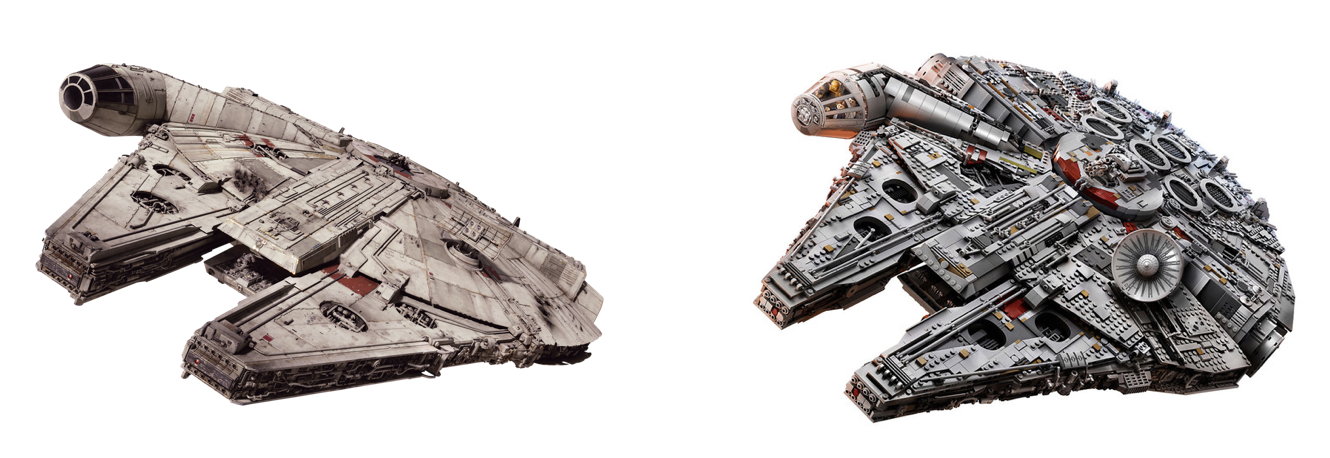
\includegraphics[width=\textwidth]{figures/MillenniumFalcon.png}
\end{figure}
These ingredients come together through a tool called a Feynman diagram.

\section{Diagrammar}

Fig.~\ref{fig:ee:gamma:gamma:example} is an example of a Feynman diagram.
\begin{marginfigure}%[th]
    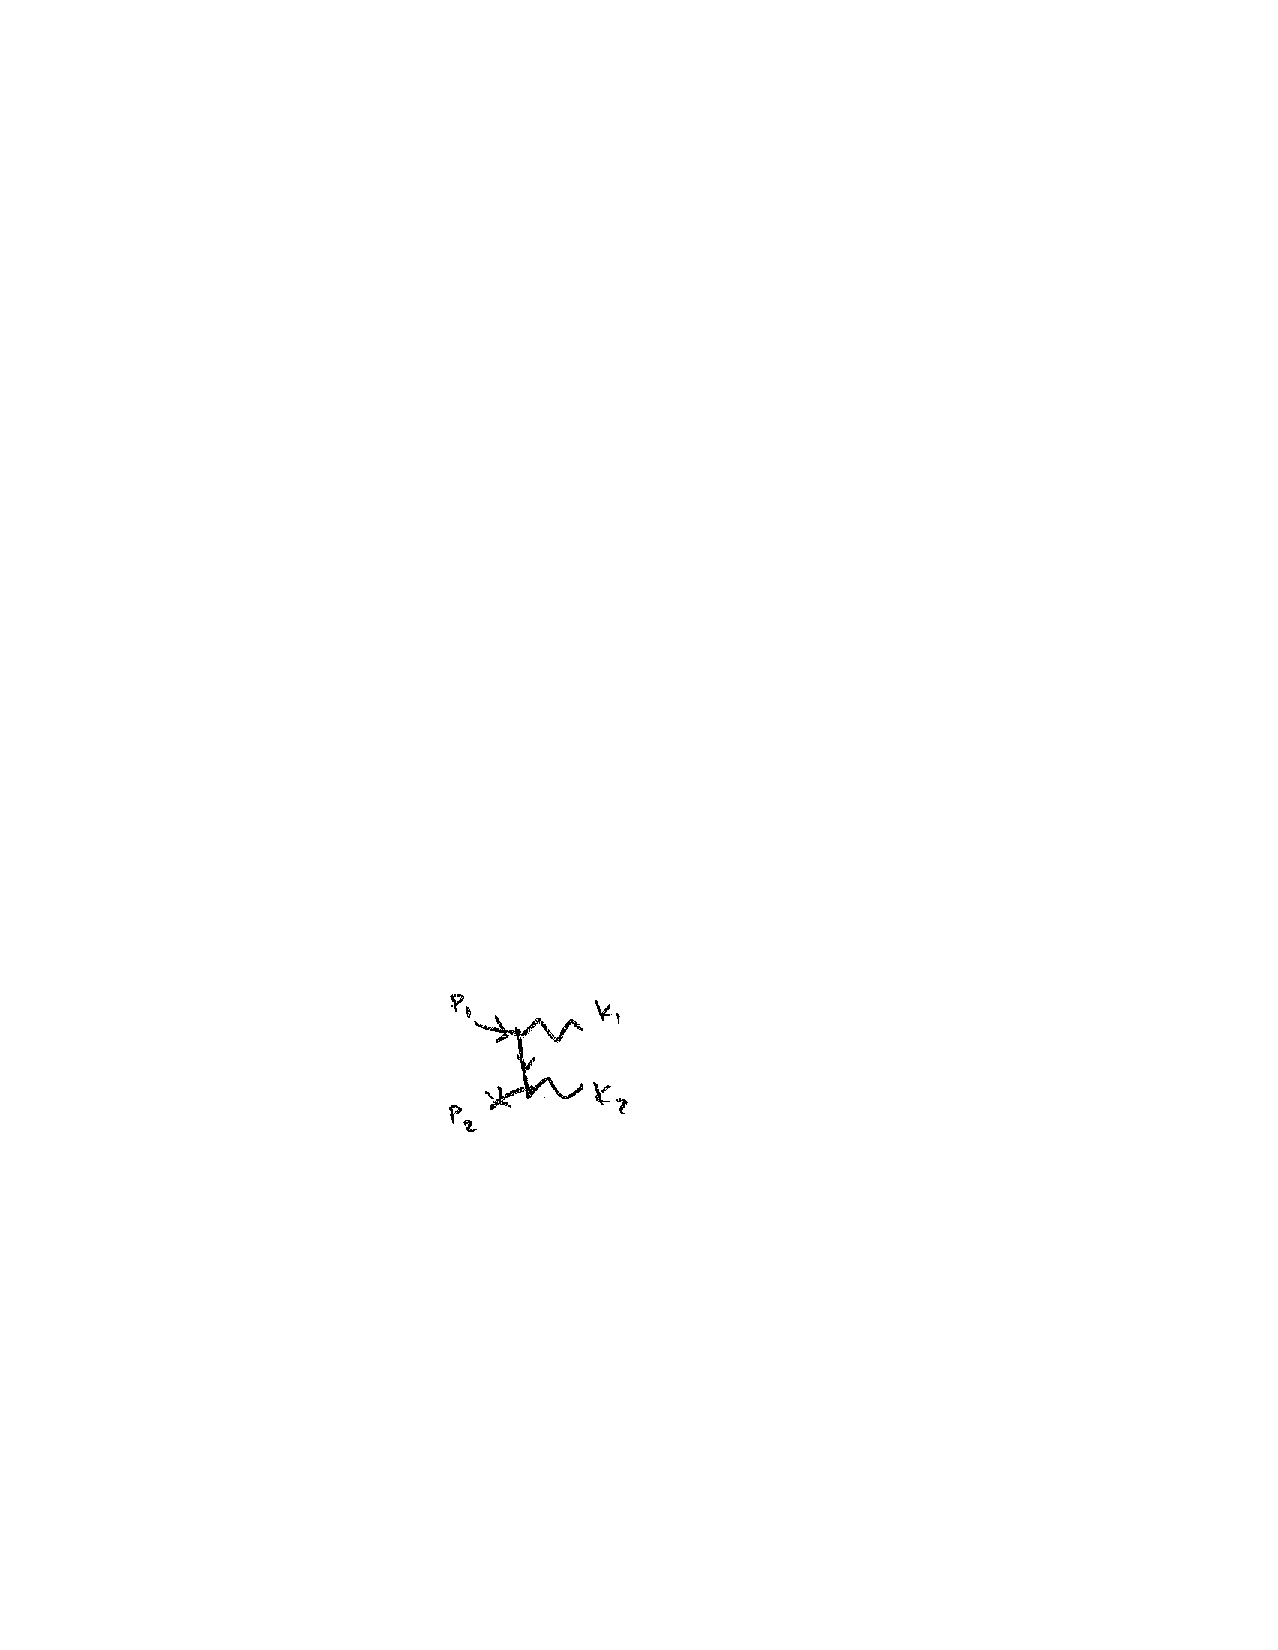
\includegraphics[width=.8\textwidth]{figures/feyn_eegaga.pdf}
    \captionsetup{font={scriptsize,sf}}
    \caption{Example of a Feynman diagram. Here an electron and a positron annihilate into a pair of photons.}
    \label{fig:ee:gamma:gamma:example}
\end{marginfigure}
Feynman diagrams are a perturbative expansion of the quantum mechanical amplitude for a something to happen. You may recall that the quantum amplitude is a ``square root of the probability\footnote{This notion comes from quantum mechanics where the probability of observing a state $\ket{\Psi}$ is $\langle \Psi | \Psi\rangle = |\Psi|^2$. In quantum field theory we typically talk about \emph{cross sections}, $\sigma$. The relation between the amplitude $\mathcal M$ and cross section is $\sigma \sim |\mathcal M|^2$ and contains kinematic factors. We determine these kinematic factors in subsequent chapters.}.'' The statement that diagrams are a \emph{perturbative expansion} means that there is some small parameter for which we are performing a Taylor expansion\sidenote{Formally the amplitudes are complex and may contain singularities. It is thus more appropriate to say that this is a \emph{Laurent expansion}. One of the `deep' ideas in quantum field theory is the intimate relationship of \emph{analyticity} (complex differentiability) to physical properties. To dig deeper, see my Physics 231 notes.\footnotemark}\footnotetext{\url{https://sites.google.com/ucr.edu/p231/}}. In the standard case, this perturbative expansion is usually an expansion in couplings.

By \textbf{coupling} I mean a parameter of the theory that determines how much some particles interact with each other. When the coupling is large, the interaction is very strong. When the coupling is small, the interaction is very weak. One coupling that you may be familiar with is the electrodynamic coupling, $e$. You are probably most familiar seeing $e$ as an ingredient in the fine structure constant, 
\begin{align}
    \alpha = \frac{1}{\hbar c \varepsilon_0} \frac{e^2}{4\pi} \approx \frac{1}{137} \ .
\end{align}
The first factor of $(\hbar c \varepsilon_0)^{-1}$ are relics of using silly units. When we use natural units---see Sec.~\ref{sec:units:dimensions}---these are set to one. You can see that $1/137$ is a small number, so it at least makes sense that if we had some amplitude $\mathcal M(\alpha)$ that is a function of the electrodynamic couplings through $\alpha$ that we could imagine doing the perturbative expansion
\begin{align}
    \mathcal M = \mathcal M_0 + \alpha \mathcal M_1  + \alpha^2 \mathcal M_2 + \cdots \ ,
    \label{eq:amplitude:perturbative:expansion}
\end{align}
and then dropping any subleading terms since we expect them to be percent-level corrections. If the couplings are large, then this expansion breaks down because subsequent terms are not small. In fact, this is what happens with the strong interactions (quantum chromodynamics), the force that holds nuclei together. Thus there are regimes where the usual Feynman expansion fails: it seems like we should not use these diagrams to describe the interactions of the quarks and gluons that are `inside' a proton.
\begin{example}
I seem to have implied that Feynman diagrams do not work for the strong interaction. Despite this, collider physicists working on the Large Hadron Collider `speak' the language of Feynman diagrams. They'll even draw diagrams that involve the strong force. What gives? Apparently I haven't told you the whole story...
\end{example}
Note that I wrote \emph{couplings} not the common phrase \emph{coupling constants}. That is because---brace yourselves---these couplings are generally \emph{not} constant. In fact, they depend on the energy scale at which you probe them. If I smash together color-charged particles\sidenote[][]{In this class and in this field, we write \emph{colored} to mean color-charged, or charged with respect to the strong force. See Chapter~5 of \emph{The Disordered Cosmos} for an anthropological discussion.\footnotemark}\footnotetext{\cite{prescod2021disordered}} at high energies, the analogous fine structure parameter for the strong force, $\alpha_\textnormal{s} = g_\textnormal{s}^2/4\pi$ depends on the characteristic energy scale\footnote{We write $\sqrt{Q^2}$ rather than $E$ because $Q^2$ is a Lorentz-invariant quantity, as we explain below in our review of special relativity.} $\sqrt{Q^2}$ at which one probes the interaction, see Fig.~\ref{fig:aS:running:from:1604.08082}. 
\begin{marginfigure}%[th]
    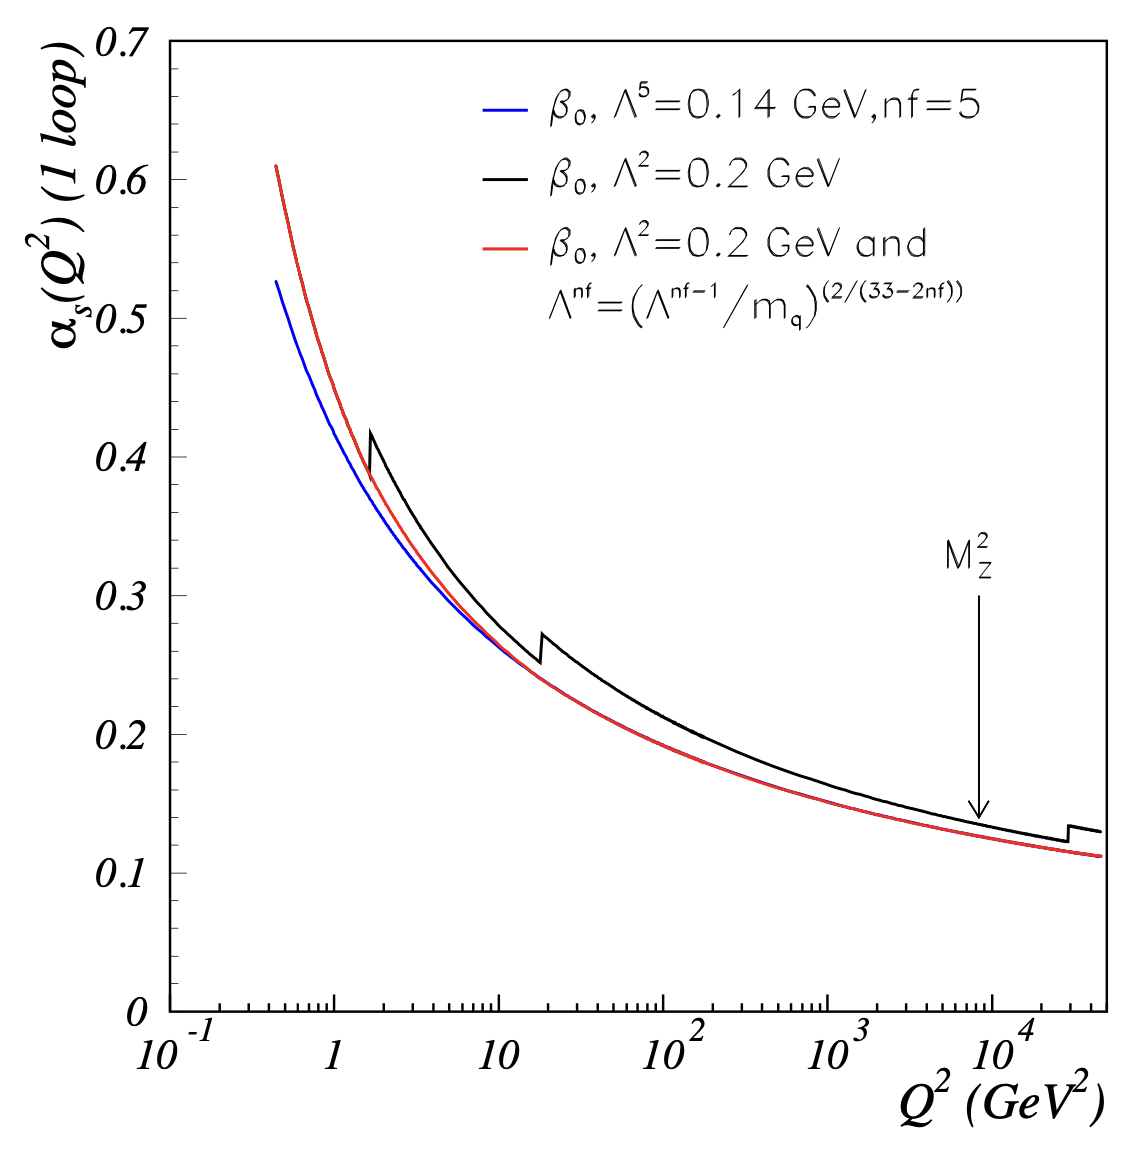
\includegraphics[width=.8\textwidth]{figures/aSrun_1604.08082.png}
    \captionsetup{font={scriptsize,sf}}
    \caption{Approximate value of the strong force fine structure parameter, $\alpha_\textnormal{s}$. Lines correspond to slightly different calculations. The horizontal axis is the square of the characteristic energy scale at which $\alpha_\textnormal{s}$ is being measured. From Fig.~3.2 of \arXiv{1604.08082}.}
    \label{fig:aS:running:from:1604.08082}
\end{marginfigure}
This idea should be shocking the first time that you see it. The `coupling constants' are not constant at all. The meaning of this oddity is an idea called \emph{renormalization} and is rooted in making sense of what the \emph{actual} small parameter is in perturbation theory: it turns out not to be the fine structure constant, but the fine structure constant times a function of the kinematics of a process. This means that at sufficiently high energies, we can meaningfully talk about Feynman diagrams of quarks exchanging gluons. However, at low energies, these diagrams lose their meaning. If you were paying attention in the previous sub-section, this is the regime where particle physics becomes nuclear physics.
\begin{example}
This reminds me of the difference between a \emph{physicist} and a \emph{physics fan}. A physics fan is someone who thinks that $1/137$ is a fundamental constant of the universe and so should be tattooed on their body. A physicist stops to think: \emph{Where does this number come from?} and proceeds to learn about the scale-dependence of the electric coupling. In fact, in this course you will find that the electric coupling is not even a fundamental parameter but a combination of more fundamental parameters. I do not care whether or not you are a physics fan, but my goal is to train you as a physicist.
\end{example}

\begin{exercise}
On the subject of couplings: is the gravitational coupling \emph{large} or \emph{small} relative to the electromagnetic coupling? You may recall from popular physics that one of these is [surprisingly?] much stronger than the other. Try to make this quantitative by comparing two numbers. \textsc{Hint}: this is a bit of a trick question. Try writing out the gravitational fine structure constant and argue why it appears that you cannot meaningfully compare it to the electromagnetic coupling.
\end{exercise}

Feynman diagrams are graphs that represent a mathematical expression for a complex number. The graphs are trajectories in spacetime that we read from left to right. Each line in a diagram represents a particle. The lines may have decorations or labels that indicate their identity. In Fig.~\ref{fig:ee:gamma:gamma:example} the two lines on the left are an electron and a positron. The two wiggly lines on the right are each photons. Each vertex (intersection of lines) represents a factor of the coupling. In Fig.~\ref{fig:ee:gamma:gamma:example} the two vertices mean that this diagram contains two powers of the electric coupling, $e$. Thus this diagram contributes to the $\mathcal O(e^2) = \mathcal O(\alpha)$ term in the expansion of the amplitude $\mathcal M(e^+e^-\to \gamma\gamma)$ in \eqref{eq:amplitude:perturbative:expansion}. The notation $\mathcal M(e^+e^-\to \gamma\gamma)$ simply means the amplitude for an electron $e^-$ and a positron $e^+$ to turn into two photons, $\gamma\gamma$.

Something else that may be familiar from quantum mechanics: amplitudes sum together. This is the origin of quantum interference and all of the fun parts of quantum physics. Our perturbative expansion \eqref{eq:amplitude:perturbative:expansion} is one example of such a sum. However there are usually multiple diagrams that contribute at a given order in perturbation theory. One of the brilliant things about these diagrams is that they have a complementary interpretation: as a \emph{sum over histories}. This is an idea that we emphasize in our review of quantum mechanics, but the idea is this: 
\begin{quote}
The amplitude to go from some initial state to some final state is represented by the sum of all Feynman diagrams that connect the initial state to the final state. Each individual Feynman diagram in the sum represents a possible history that the initial state could have taken to reach the final state.
\end{quote}
This sum over histories interpretation is outrageous the first time you see it but is ultimately an extension of the principle of least time that underlies Snell's law in optics. The generalization to a principle of least action is the core of Lagrangian mechanics and was in fact Feynman's Ph.D thesis\autocite{feynman2005feynman}. 

The diagrams are simply a tool. Feynman's long time physics rival and co-Nobel prize winner, Julian Schwinger, was a master of calculating amplitudes in quantum field theory \emph{without} any diagrams. In one interpretation of history, Feynman's main contribution at this stage of physics history was bringing that calculational technology to the masses by giving each term an intuitive meaning.\sidenote{It is no surprise that he is also (mis-)attributed as the spokesperson of the ``shut up and calculate'' school of quantum physics.\footnotemark}\footnotetext{\cite{10.1063/1.1768652}} Veltman has a nice physics-oriented history of the spread of Feynman diagrams in his book \emph{Diagrammatica}\autocite{Veltman:1994wz}. This book should not be confused with a set of lecture notes he co-wrote with 
't~Hooft called ``Diagrammar\autocite{tHooft:1973wag},'' which inspired the name of this section.
% Not for this class, but also interesting: https://arxiv.org/abs/2109.06889
% Diagrammar of physical and fake particles and spectral optical theorem
%  Anselmi


As a final note: there is far more to quantum field theory than Feynman diagrams. As a perturbative expansion, Feynman diagrams represent the \emph{easiest} part of quantum field theory. But just as there are functions that cannot be meaningfully Taylor expanded\sidenote{Try expanding $\exp(-x^{-2})$ around the point $x_0 = 0$. Every term at every order vanishes, even though the function is well defined and non-zero away from the origin. The quantum field theory analog is something called an instanton and is beyond the scope of this course.}, there are vast swaths of field theory that are intrinsically \emph{non-perturbative}. Quantum chromodynamics at low energies---where we must turn to methods in nuclear physics---is one example. We make this caveat to emphasize that although we lean heavily on the diagrammatic interpretation of particle physics, we are still just scratching the surface.



% HW: muon shot. 
% Idea: every homework is a story



\section{Kinematics and Dynamics}

I may be the only person who makes a big deal about this, but we can separate our study of particle physics into two parallel tracks: {kinematics} and {dynamics}. You probably know that these words ``have to do with physics,'' but the distinction between them is rarely delineated. In fact, I suspect I may be making it up---in which case, here are the working definitions for this class. 

\textbf{Kinematics}\index{kinematics} has to do with the motion of particles through space and time. The kinematics of a scattering process relates to the momentum and energy of those particles. The conservation of energy and momentum are also kinematical facts\sidenote{Though their derivation through Noether's theorem is arguably a statement about dynamics.}. The thread of physics that is most relevant to this study is \emph{relativity}, and in particular the flat-spacetime version known as \emph{special relativity}.\sidenote{In contrast, general relativity is the study non-flat spacetimes. One can argue that it is the \emph{dynamics} of spacetime itself.}

\textbf{Dynamics}\index{dynamics}, on the other hand, has to do with the rules for how particles interact. When we talk about a theory or a model of particle physics, we usually mean a description of the dynamics. These are encoded in the action or Lagrangian of a theory. The dynamics of a theory draws primarily from the rules of \emph{quantum mechanics}.

Feynman diagrams are an output of the dynamics of a theory. However, a Feynman diagram is only physically meaningful if it obeys the rules of the kinematics of a theory. Kinematics are an additional consideration when we convert the squared amplitude into something physically measurable.
\begin{example}
You can draw a Feynman diagram for a process like $\gamma \to e^+e^-$ by which a photon decays into an electron--positron pair. You could even calculate the amplitude for this process to happen. However, this process is kinematically forbidden because it cannot simultaneously conserve energy and momentum. The amplitude is nonzero, but the decay rate is forced to be zero by kinematics.
\end{example}
\begin{exercise}
Show that both energy and momentum cannot be conserved in $\gamma \to e^+e^-$. There are many ways to do this, including some that are more slick than others. If you are stuck, come back to this exercise after our review of special relativity.
\end{exercise}

In this course, you can think of dynamics as the set of rules\sidenote{Called \emph{Feynman rules}.} that tell us how we may construct Feynman diagrams. These rules are an encoding of the Lagrangian of the theory.  You can think of kinematics as conditions on the energies and momenta of the initial and final states of an amplitude---these are the external lines of a diagram. Notably, kinematic constraints do not apply to the particles on the \emph{inside} of a Feynman diagram. Lines that obey the kinematic constraints are called \textbf{on shell}, while those that do not are called \textbf{off shell}.\sidenote{What is the \emph{shell}? It is the hypersurface the four-dimensional space of energy and momentum that satisfies the Einstein relation, $E^2 = m^2c^4 + p^2 c^2$ for a particle of mass $m$, energy $E$, and three-momentum $p$.} With this jargon, we say that external lines on a Feynman diagram represent parts of the initial or final states of a process and must be on shell. Internal lines are, in general, off shell.

\subsection{Symmetry}

The notion of \emph{symmetry} plays a central role for both the kinematics and the dynamics. The mathematical description of symmetry is called group theory and the way in which symmetries act on objects is called representation theory.\sidenote{I am name-dropping subjects because I am often asked what subjects should an aspiring theoretical physicist master.} The tables of Clebsch--Gordan coefficients that you may have invoked in your study of addition of angular momentum in quantum mechanics is an output of the representation theory of the group of three-dimensional rotations. In this course we are specifically interested in the representation theory of continuous groups---symmetries like rotations where you can transform by an arbitrary amount---called \emph{Lie groups}.\sidenote{Pronounced `lee.'} As humble physicists\sidenote{Oppenheimer: Well, if that’s how you treat a lieutenant colonel than I hate to see how you treat a humble physicist.\\Leslie Groves: If I ever meet one I'll let you know. (From \emph{Oppenheimer}, 2023)} the way we work with symmetries is to introduce indices. Objects that carry these indices are called \textbf{tensors}.

In special relativity (kinematics) the simplest tensors are four-vectors. They are called four-vectors because they are vectors that have four components. For example, the four-momentum of a particle may be written $p^\mu$. The index is $\mu$. There is a related object called $p_\mu$ with a lower index. These are related by a tensor called the metric tensor, which for our purposes we write $\eta_{\mu\nu}$. The metric gives us a way to define an inner product. This should all sound familiar from linear algebra because this \emph{is} linear algebra. In representation theory, the objects that get rotated\sidenote{By `rotate' I mean a general symmetry transformation. For the case of special relativity, one can have boosts in addition to rotations.} are vectors in a vector space. If you ever wonder why I teach Physics 17 the way that I do, it is because I want students to be primed to understand representation theory as it appears in physics.

Maybe the phrase `inner product' caught your ear. This is the same idea that comes up in quantum mechanics. In fact, now you may recall that quantum mechanics really boils down to complex linear algebra. In fact, many ideas in quantum mechanics are ultimately group theoretical. For example, the commutator is the natural multiplication operation between elements of a group.\sidenote{Check that while this may be surprising, it is sensible. The commutator of two operators is another operator in the same way that the multiplication of two things of a given type should be another thing of the same type.} Furthermore, finite transformations are the exponentiation of infinitesimal transformations. For example, the Hamiltonian $\hat H$ is the generator of translations in time. A finite translation in time is
\begin{align}
    \hat U(t) = e^{-i \hbar t\hat H} \ .
    \label{eq:Ut:time:H}
\end{align}
\flip{check the $\hbar$}
In particle physics we will meet several \textbf{internal symmetries} that mathematically describe the rotation of an object in different vector spaces. These do \emph{not} correspond to spacetime rotations or boosts. Instead, they may represent a rotation between quarks of different color charges.\sidenote{We define these carefully below where we discuss quantum chromodynamics. For this introduction just humor me and go with the flow to appreciate the big idea.} The infinitesimal generators of these transformations take the form\footnote{I am using `physicist' shorthand here and referring to a tensor by its components. Supercilious mathematicians sneer at us for this. Formally, $A\aij{i}{j}$ is not a matrix, it is the $i$--$j$ \emph{component} of a matrix A. Physicists justify our sloppiness because anyone who is paying attention should understand what we mean and, more importantly, by keeping the indices explicit we can see how the tensor transforms.}
\begin{align}
(T^A)\aij{i}{j}\ ,    
\end{align}
where we recognize three indices. The index $A$ is called an adjoint index and tells you which direction you are rotating. For the rotation group, $A$ takes values from 1 to 3 corresponding to rotations about the $x$, $y$, and $z$ axes. All other rotations are combinations of these. The other two indices, $i$ and $j$ depend on the \emph{representation} of the object that we are rotating. 
\begin{example}
In quantum chromodynamics we there are eight generators of so-called color symmetry. This means $A$ takes values from 1 through 8. This group is called \acro{SU(3)}, which stands for the set of $3\times 3$ special unitary matrices.\sidenotemark A quark has indices that I conventionally write with lowercase letters from the middle of the Roman alphabet that take values $m$ from 1 to 3 corresponding to red, blue, and green. The matrix $(T^4)\aij{m}{n}$ represents a particular rotation around the $A=4$ axis. A finite transformation by angle $\theta$ takes the form 
\begin{align}
    q^m \to \sum_n e^{i \theta (T^4)\aij{m}{n} } q^n \equiv \sum_n U(\theta)\aij{m}{n}q^n \ ,
\end{align}
where the sum over $n$ is what we expect from matrix multiplication.
\end{example}\sidenotetext[][]{Special means unit determinant. Unitary, as you may recall from quantum mechanics, means that the hermitian conjugate is its inverse.}

This is all to say that indices feature front-and-center in this course. They are a crutch for us to talk about the underlying symmetries that govern both the kinematics and dynamics of particle physics. We will spend a good chunk of this course building familiarity with how to interpret and manipulate indices. This is a mathematical skill that is far more general than particle physics itself.





\section{Natural Units}
\label{sec:units:dimensions}

By this stage of your physics career you are an expert at converting units. The trick is to multiply be one in different forms. Suppose you have some unit $x$ that is related to unit $y$ by some prefactor,
\begin{align}
    x = a y \ . \label{eq:unit:conversion}
\end{align}
Then you can derive that
\begin{align}
    1 = \frac{ay}{x} = {x}{ay} \ .
    \label{eq:multiply:by:one:unit:conversion}
\end{align}
Then if some quantity is, say, $3.4\,x$, you know that you can write it out in terms of $y$ simply by multiplying by one, cleverly written:
\begin{align}
    3.4\,x = 3.4\times 1 \times x = 3.1 \times \frac{ay}{\cancel{x}} \times \cancel{x}
    = (3.4a)\, y \ .
\end{align}
\eqref{eq:multiply:by:one:unit:conversion} tells us that there is a universal, unambiguous constant ratio that relates unit $x$ to unit $y$. 


\begin{example}
Suppose someone tells you the number of feet in a mile,
\begin{align}
    1~\text{mile} = 5280~\text{feet} \ .
\end{align}
This number just so happens to be the mass of the $B$ meson in \acro{MeV}.
You can derive that
\begin{align}
    1 = 5280~\frac{\text{feet}}{\text{mile}}
    = \frac{1}{5280}~\frac{\text{mile}}{\text{feet}} \ .
\end{align}
From this you can deduce that a distance of $1.5$ miles is
\begin{align}
    1.5\,\text{mile} = 
    1.5\,\cancel{\text{mile}} \times \left(5280~\frac{\text{feet}}{\cancel{\text{mile}}}\right) = 
    7920~\text{feet} 
    \approx 8000~\text{feet} 
    \ .
\end{align}
\end{example}

If this all looks completely simple then \emph{good}, it is supposed to. There is nothing deep or mysterious about changing units. Let us really put it to work. \textbf{Natural units}\index{natural units} are a convenient choice that boils down to the following identifications:
\begin{align}
    c &=1  &
    \hbar &= 1
    \ .
\end{align}
That's right. The speed of light $c$ and reduced Planck's constant $\hbar$ are set to one. This may bother you. After all, you know from past coursework that these are \emph{not} dimensionless quantities:
\begin{align}
    c &= 3\times 10^{8}\,\frac{\textnormal{m}}{\textnormal{s}}
    &
    \hbar &= 1\times 10^{-34}\,\frac{\textnormal{m}^2 \textnormal{kg}}{\textnormal{s}} \ .
    \label{eq:c:hbar:SI}
\end{align}
Setting $c = 1$ would then mean that there is an unambiguous way conversion between length and time, as if these were measuring the ``same thing.'' But length is measured by rulers and time is measured by clocks: how are these the same? They are the same \emph{precisely} because nature\sidenote{All our observations since the Michelson--Morley experiment are consistent with a constant speed of light and this is built into our theory of special relativity. Theoretically this is an aesthetic unification of space and time that laid the foundation of general relativity, which in turn has passed every experimental prediction.} gives us a universal, unambiguous constant ratio that relates units of length into units of time. This constant is the speed of light.
\begin{example}
A lightyear is a unit of distance. It is defined to be the distance traversed by a particle traveling at the speed of light,
\begin{align}
    \text{lightyear} = c\, \text{year} \ ,
\end{align}
where we see that the speed of light in natural units $c=1$ plays the role of a conversion factor in \eqref{eq:unit:conversion}. 
\end{example}
% Naive dimensional analysis
% \autocite{Manohar:1983md,Georgi:1986kr,Georgi:1992dw}
Identifying the speed of light as a conversion factor ends up relating another set of dimensionful quantities. All velocities in natural units are dimensionless. This is because we can simply write any velocity in units of the speed of light.
\begin{example}
The tangential speed of the Earth around the solar system is around $v = 200$\,km/s. In natural units this is a dimensionless number:
\begin{align}
v = 200\,\frac{ \textnormal{km} }{ \textnormal{s} }
=
2\times 10^{5} \, \frac{\textnormal{m}}{\textnormal{s}} 
\times 
\left(\frac{1}{3\times 10^8}\frac{\textnormal{s}}{\textnormal{m}}\right)
= 7 \times 10^{-3} \ .
\end{align}
In natural units, any sensible velocity has magnitude less than one. Otherwise something is traveling faster than the speed of light. 
\end{example}
\begin{exercise}
What goes wrong in physics if a particle can travel faster than the speed of light? \textsc{Hint}: review the relativity of simultaneity. 
\end{exercise}
Velocities are dimensionless in natural units. 
Recall that energy has the units of mass times velocity squared. You may recall this from from 
\begin{align}
    E_\textnormal{kinetic} = \frac{1}{2} mv^2 \ .
\end{align}
You may argue that this formula is only true for kinetic energy. That is true, energy---no matter what the form---is carries the same type of dimension. Because velocities are dimensionless, then the dimensions of energy and the dimensions of mass must be the same. In other words, mass and energy are ``the same thing.'' Given a particle of some mass---say the mass of a proton, $m_\textnormal{p}$---there is an associated energy that is $m_\textnormal{p} \times 1  = m_\textnormal{p} c^2$. This looks remarkably like the non-relativistic limit of the Einstein relation,
\begin{align}
    E = mc^2 \ .
\end{align}
Indeed, in that limit, the Einstein relation just tells us that mass and energy are the same thing. The square of the speed of light plays the role of a conversion factor between them. It is conventional for particle physicists using natural units to measure everything in units of energy. A particularly useful energy scale is 
\begin{align}
    m_\textnormal{p} = 1\,\text{\GeV{}} \ .
\end{align}
To one significant figure, the mass of the proton happens to be about one billion times an electron volt.  
\begin{exercise}
How much do you weigh in \GeV{}? 
\end{exercise}
Sometimes we lapse into other powers of electron volt. Some useful values are the mass of the electron and the mass of the Higgs boson\sidenote{We write $m_h$ to three significant figures because the Higgs is a big deal.}, and the center-of-mass energy of proton-proton collisions at the Large Hadron Collider:
\begin{align}
    m_e &= 0.5\,\text{MeV}
    &
    m_h &= 125\,\text{GeV}
    &
    E_\text{cm} &= 14\,\text{TeV} \ .
\end{align}



What about $\hbar = 1$? Planck's constant carries units of angular momentum\sidenote{These are also the units of action, $S=\int dt\,L$.}, or energy times time. Using the just-established equivalence of mass and energy in natural units, this tells us that
\begin{align}
    \hbar &= 7 \times 10^{-22}\,\textnormal{MeV}\,\textnormal{s}  \equiv 1 \ . 
\end{align}
% \begin{align}
%     \hbar = 10^{-34}\,\frac{\textnormal{m}^2 \textnormal{kg}}{\textnormal{s}}
%     \times 
%     \left(3\times 10^{8}\,\frac{\textnormal{m}}{\textnormal{s}}\right)^{-2}
%     = 
%     10^{-51}\,\textnormal{kg}\,\textnormal{s} \ .
% \end{align}
This means that the fundamental unit of ``quantum-ness'' tells us that time and inverse energy are ``the same thing.'' At this point, you can multiply and divide by $c$ and $\hbar$ as needed to write all dimensionful parameters in units of \GeV{} to some power. 
\begin{example}
An additional conversion is to set the Boltzmann factor, $k_\textnormal{B} =1$. This is the observation that thermal energy is energy and can be measured in \GeV{}.
\end{example}
We provide a useful table for conversions to one significant figure.
\begin{table}[ht]
    \renewcommand{\arraystretch}{1.3} % spacing between rows
    \centering
    \sidecaption[Useful conversions to natural units. Adapted from Palash Pal's website.][-2\baselineskip]{%
        Conversion of units using $\hbar = c = k_\textnormal{B} = 1$. The row heading is equal to the table entry times the column heading so that a \GeV{} is a small number of Planck masses, $M_\textnormal{Pl}$.  Adapted from Palash Pal's website.\footnotemark 
  %       \label{table:app:natural:unit:conversion}
    }
    \begin{tabular}{ @{} lllllll @{} } \toprule % @{} removes space
        & \GeV{} & g & K & cm$^{-1}$ & sec$^{-1}$ & M$_\textnormal{Pl}$
        \\ \midrule
        \GeV{} % col
        & % GeV
        & 1$\times 10^{-24}$ % g
        & 1$\times 10^{13}$% K
        & 5$\times 10^{13}$% cm-1
        & 2$\times 10^{24}$% s-1
        & 8$\times 10^{-20}$% Mpl
        \\
        g % col
        & 6$\times 10^{23}$% GeV
        & %$\times 10^{}$% g
        & 7$\times 10^{36}$% K
        & 3$\times 10^{37}$% cm-1
        & 9$\times 10^{47}$% s-1
        & 5$\times 10^{4}$% Mpl
        \\
        K% col
        & 9$\times 10^{-14}$% GeV
        & 2$\times 10^{-37}$% g
        & %$\times 10^{}$% K
        & 4%$\times 10^{}$% cm-1
        & 1$\times 10^{11}$% s-1
        & 7$\times 10^{-33}$% Mpl
        \\
        cm$^{-1}$ % col
        & 2$\times 10^{-14}$% GeV
        & 4$\times 10^{-38}$% g
        & 2$\times 10^{-1}$% K
        & %$\times 10^{}$% cm-1
        & 3$\times 10^{10}$% s-1
        & 2$\times 10^{-33}$% Mpl
        \\
        sec$^{-1}$ % col
        & 7$\times 10^{-25}$% GeV
        & 1$\times 10^{-48}$% g
        & 8$\times 10^{-12}$% K
        & 3$\times 10^{-11}$% cm-1
        & %\times 10^{}$% s-1
        & 5$\times 10^{-44}$% Mpl
        \\
        M$_\textnormal{Pl}$% col
        & 1$\times 10^{19}$% GeV
        & 2$\times 10^{-5}$% g
        & 1$\times 10^{32}$% K
        & 6$\times 10^{32}$% cm-1
        & 2$\times 10^{43}$% s-1
        & %$\times 10^{}$% Mpl
        \\ \bottomrule
    \end{tabular}
  %   \caption[Useful conversions to natural units. Adapted from Palash Pal's website.]
  %   {
  %       Conversion of units using $\hbar = c = k_\textnormal{B} = 1$. The row heading is equal to the table entry times the column heading so that a \GeV{} is a small number of Planck masses, $M_\textnormal{Pl}$.  Adapted from Palash Pal's website.\footnotemark 
        \label{table:app:natural:unit:conversion}
  % }
\end{table}\footnotetext{\url{https://www.saha.ac.in/theory/palashbaran.pal/conv.html}}

\begin{example}[Mnemonics]
You can use your favorite equations in physics as mnemonics for natural units. We already saw how $E=mc^2$ reminds us that energy and mass both carry the same units. You can also invoke Heiseinberg's uncertainty relations
\begin{align}
    \Delta x\,\Delta p &\sim \hbar 
    &
    \Delta E \Delta t &\sim \hbar
\end{align}
to remind us that momentum and distance carry reciprocal units, as do energy and time. Because $c=1$ tells us that distance and time are the same, we find
\begin{align}
    \text{length} \sim \text{time} \sim \frac{1}{\text{mass}} 
    \sim \frac{1}{\text{energy}} \ .
\end{align}
\end{example}

The great thing about natural units is that we just have to keep track of one unit, say \GeV{}. Dimensional analysis is very simple and we introduce the bracket notation:
\begin{align}
    [x] \defeq ``\text{dimensions of }x \ .''
\end{align}
$[x]$ means: what power of energy is the unit of quantity $x$?
\begin{example}
For a distance $\ell$, time $t$, mass $m$, and energy $E$:
\begin{align}
    [\ell] &= -1
    &
    [t] &= -1
    &
    [m] &= 1
    &
    [E] &= 1
    \ .
\end{align}
\end{example}
\begin{exercise}
What are the dimensions of the gravitational constant, $[G_\textnormal{N}]$? \textsc{Hint}: you can use the force law for gravity to figure out the \acro{SI} units of $G_\textnormal{N}$.
\end{exercise}

\begin{exercise}
Show that the units of action are the same as the units of angular momentum. \textsc{Hint}: use the expression for the action with your favorite choice of Lagrangian.
\end{exercise}

\begin{example}[Collider physics as microscopy]
The Large Hadron Collider is a microscope. The center of mass energy of t
\end{example}

\chapter{Relativity, Quantum Mechanics}

We begin our study of particle physics with a lightning review of selected topics in special relativity and quantum mechanics.

\section{Kinematics}

The popular Einstein relation, $E = mc^2$, is actually the low [kinetic] energy limit of the `full' relation:
\begin{align}
    E^2 = m^2 c^4 + \vec{p}^2 c^2 \ .
    \label{eq:Einstein:relation:plus}
\end{align}
Equations that relate energy to momentum show up all over physics and have a special name: \textbf{dispersion relations}.\sidenote{As a student I always found this name intimidating because it would keep showing up in very different and increasingly advanced corners of physics. I felt like I must be missing something deep, especially since the word \emph{dispersion} did not seem to obviously fit. Historically, these relate wavelength to frequency. Recall that wave velocity is the product of wavelength and frequency---but wave velocity is purely a property in medium. Wavelength (or wave number) is directly related to momentum---think 
$\sin(kx)$---while frequency is directly related to energy---think $E=\hbar\omega$. These of these parameters are related to absorption (or decay) through complex analysis; these are the celebrated Kramers--Kr\"onig relations. We mention all of this to encourage you to look these ideas up and see how they connect; they are one of the deep threads in physics.} 
\begin{exercise}
It is obvious that \eqref{eq:Einstein:relation:plus} reproduces $E=mc^2$ when $\vec{p}=0$. Show that the leading order correction in the small-$\vec{p}$ limit is simply the non-relativistic kinetic energy of the particle. \textsc{Hint:} start by identifying the \emph{dimensionless} small parameter and Taylor expand.
\end{exercise}
In natural units we set $c=1$. In this relation, $m$ is the mass of a particle while $E$ and $\vec{p}$ are the energy and three-momentum respectively. Let us write this with the kinematic quantities on the same side of the equation:
\begin{align}
    m^2 = E^2 - \vec{p}^2 \ .
\end{align}
A particle that satisfies this relation is said to be \textbf{on shell}\index{on shell} or \emph{physical}. Anticipating quantum mechanics, another way of saying this is that on shell particles are \emph{observable states}. Personally, I think of `on shell' states as being \emph{nice} states that are relatable to my ordinary human experiences. This is in contrast to \textbf{off shell} particles, which states that are \emph{not} on shell and are intrinsically quantum. Off shell states are not observable and do not make sense classically. 

A scattering process is one where some number of \emph{observed} initial state particles interact quantum mechanically and produce and \emph{observed} number of final state particles. These initial and final states must each be on shell and conserve energy and momentum. 
\begin{newrule}[Kinematics]
A \textbf{physical scattering process} is one with an on shell initial state and an on shell final state. This just means that each particle in the initial and final state are on shell. Furthermore, the total energy $E$ and total three-momentum $\vec{p}$ are conserved through the process. In equations:
\begin{align}
    E_\textnormal{in} &= E_\textnormal{out}
    &
    \vec{p}_\textnormal{in} &= \vec{p}_\textnormal{out}
    &
    m_i^2 = E_i^2 - \vec{p_i}^2 \ ,
\end{align}
where $i$ labels each of the external (initial or final) particles. Technically, we should also specify that $E_i>0$, but for us we can take this as an ``obvious'' fact.\sidenotemark Note that in this notation, $E_\textnormal{in}$ is the sum of the energies of all the initial state particles, and similarly for the other in/out quantities.
\end{newrule}\sidenotetext{From a group theory perspective, positive energy means that we are restricting to the \emph{orthochronus}\index{orthochronus} Lorentz group. This means that particles always move forward in time, no matter what reference frame we are in. The relation between energy positivity and direction in time should be clear from the time evolution operator, \eqref{eq:Ut:time:H} with $\hat H\to E$.}

Suppose you have a particle detector that measures the energy of a particle passing through it---this is called a \emph{calorimeter}. If you also know the mass of the particle, then you can also unambiguously determine the magnitude of the momentum, $|\vec{p}|$.  Alternatively, if you could separately measure the energy and the momentum of a particle, then you can unambiguously infer its mass. This is all obvious because you are using one Einstein relation to relate three variables---mass, energy, and momentum. 

\begin{exercise}
Suppose you have a process where one particle decays into two other particles; these particles do not necessarily have the same masses, but suppose you know all of the masses. You know the energy and momentum of the initial particle, $E_\textnormal{in}$ and $\vec{p}_\textnormal{in}$. You do not know, \emph{a priori}, the energies or momenta of the final state particles. How many unknown scalar quantities are there? How many constraint equations are there? \textsc{Hint}: recall that $\vec{p}$ is a vector with three separate quantities. Argue that there is generically \emph{no} solution to this system unless some parameters (e.g.\ the masses) are just right.
\end{exercise}

\begin{exercise}
Suppose you have a process where two particles come in, and two particles come out. The particles do not necessarily have the same mass, but you know all of the masses. If you know the energies of the initial particles, how many unknowns are there and how many constraint equations are there? Do you expect this system to have a solution? \textsc{Note}: for the purposes of this problem, assume that all energies are positive. This corresponds to satisfying the orthochronus constraint. If you are nervous about this, check that by increasing the energies of the initial particles you can make sure that the final state particles have positive energy. 
\end{exercise}


\section{Special Relativity}

\begin{flipcomment}
This section is a very brief review of the main points. For a more systematic derivation, please see my Physics 17 lecture notes. 
\end{flipcomment}

...
\autocite{bais2007very}

\section*{Acknowledgments}

\acro{PT}\ thanks 
all the people who taught him quantum field theory and particle physics over the years. In particular, courses from Scott Thomas, Pat Burchat, Savas Dimopoulos, Aaron Roodman, Michael Peskin, Shamit Kachru, David Tong, Maciej Dunajski, Ben Allanach, Hugh Osborn, Fernando Quevedo, Silvia Pascoli, Csaba Cs\'aki, Maxim Perelstein, and Yuval Grossman. I am further indebted to those who were (and are still) on this journey to figure this all out---those are too many to list explicitly, but I especially thank my postdoctoral mentors Tim Tait and Jonathan Feng, and everyone who has ever shared an office or done problem sets with me. My approach to writing and pedagogy is inspired by the writing of Sidney Coleman, Anthony Zee, David Tong, and Matthew Strassler---the physicists who you read if they have ever written anything vaguely related to whatever it is you are trying to learn.
%
% \acro{PT} thanks 
%     the Aspen Center for Physics (\acro{NSF} grant \acro{\#1066293})
%     % and the Kavli Institute for Theoretical Physics (\acro{NSF} grant \acro{PHY-1748958})`'
%     for 
%     its 
%     % their
%     hospitality during a period where part of this work was completed. 
% %
% \acro{PT} is supported by the \acro{DOE} grant \acro{DE-SC}/0008541.
\acro{PT} is supported by a \acro{NSF CAREER} award (\#2045333).

%% Appendices
\appendix
% \chapter{Proper appendix}
% index that follows this chapter.

% \section{Things to work on}

% It may be nice to incorporate something like \texttt{classicthesis}\footnote{\url{https://www.ctan.org/tex-archive/macros/latex/contrib/classicthesis/}}


\printindex

%% Bibliography
%% USING BIBLATEX, SKIP BIBTEX
%% Use inspireHEP bibtex entries when possible
% \bibliographystyle{utcaps} 	% arXiv hyperlinks, preserves caps in title
% \bibliography{bib title without .bib}


\end{document}